% Springer LNNS (Lecture Notes in Networks and Systems) format
\documentclass{llncs}

\usepackage[utf8]{inputenc}
\usepackage[T1]{fontenc}
\usepackage{cite}
\usepackage{amsmath,amssymb}
\usepackage{graphicx}
\usepackage{booktabs}
\usepackage{array}
\usepackage{url}
\usepackage{hyperref}
\usepackage{float}

\begin{document}

\title{Evidence-Grounded Anomaly Detection and Attribution in Financial Time Series via Modular Embedder-Detector Architectures}

\author{Ngo Van Truong Phuc\orcidID{0009-0006-1654-2869} \and Ha Le Thanh Nhan\orcidID{0009-0005-1076-8720} \and Dinh Dong Tien\orcidID{0009-0008-0312-4750} \and Phan Anh Tai\orcidID{0009-0004-6399-8629} \and Le Vo Minh Thu\orcidID{0009-0008-3480-8311}}

\institute{FPT University, D1 Street, Saigon Hi-tech Park, Tang Nhon Phu Ward, 71320, Ho Chi Minh City, Viet Nam}

\maketitle

\begin{abstract}
Financial anomalies (price spikes, volatility bursts, and regime shifts) present tail risks that existing detectors cannot adequately explain. Current systems return opaque scores without identifying influential timesteps, key features, or verifiable real-world causes. We introduce an evidence-based anomaly detection and attribution framework on a modular Embedder--Detector architecture, pairing three time-series embedders (iTransformer, TimesNet, PatchTST) with two transformer-based detectors (Anomaly Transformer, TranAD), trained on 500 tickers across 11 sectors. Models are evaluated on a dual-substrate benchmark combining real trading data and synthetic Ornstein--Uhlenbeck processes across three difficulty levels. Explanations are generated via a three-layer interpretability stack: Integrated Gradients for feature attribution, Monte Carlo TimeSHAP for temporal anatomy, and LLM-ranked news retrieval for event grounding. TranAD excels at point-anomaly recall; the Anomaly Transformer maintains broader contextual sensitivity. The best configuration achieves $F_1 = 0.614$, and XAI analysis reveals mean recency concentrations of 28\% versus 70\%, directly exposing complementary temporal receptive fields.
\keywords{anomaly detection, financial time series, transformer, explainability, time-series embedder}
\end{abstract}

\section{Introduction}

Anomaly detection in financial time series is a high-stakes problem. Abnormal price behaviour (sudden spikes, volatility bursts, gap returns, and regime shifts) frequently coincides with identifiable external catalysts and carries significant tail risk for portfolio managers and regulatory oversight. Yet most deployed systems operate as black boxes: they return a scalar anomaly score but provide no mechanism for understanding why a flagged event was anomalous, which features drove the detection, or what real-world events plausibly caused it. Recent transformer-based detectors, notably the Anomaly Transformer and TranAD, alongside general-purpose time-series embedders (iTransformer, TimesNet, PatchTST) have advanced detection quality, but a key question remains: does prepending a state-of-the-art embedder to a transformer-based detector improve detection quality, and does the answer depend on the detector architecture?

Existing benchmarks compound this gap in two ways. First, they evaluate detectors in isolation, making it difficult to attribute performance differences to architectural choices. Second, most rely on a single data substrate with imprecise ground truth~\cite{ref14,ref4}, and rarely disentangle substrate effects from anomaly type. This paper focuses on transformer-based architectures; comparison against non-deep-learning baselines is left to future work.

The main contributions of this paper are as follows:
\begin{itemize}
    \item \textbf{A systematic embedder-detector pairing study:} We evaluate six Embedder $\rightarrow$ Detector combinations, pairing iTransformer, TimesNet, PatchTST, and a no-embedder baseline with Anomaly Transformer and TranAD, trained on 500 tickers across 11 sectors. Embedder benefit is architecture-conditional: the Anomaly Transformer performs best without an upstream embedder, while TimesNet provides meaningful gains for TranAD.
    \item \textbf{A dual-substrate, difficulty-stratified evaluation benchmark:} We construct two test substrates: 25 real tickers selected for minimal anomaly contamination, and fully synthetic data via Ornstein-Uhlenbeck log-price processes. Both undergo anomaly injection across Easy, Medium, and Hard difficulty tiers, surfacing a critical finding: TranAD-based models collapse in recall on mathematically pure synthetic environments.
    \item \textbf{A three-layer XAI pipeline for evidence-grounded anomaly attribution:} We apply Integrated Gradients for feature attribution, Monte Carlo TimeSHAP for temporal decomposition, and LLM-ranked news retrieval to ground detections in verifiable real-world catalysts, producing a complete interpretable account linking model internals to market microstructure features and external news narratives.
\end{itemize}

The remainder of this paper is organized as follows: related work (Sect.~2), methodology (Sect.~3), experiments and results (Sect.~4), XAI analysis (Sect.~5), discussion and limitations (Sect.~6), and conclusion (Sect.~7).

\section{Related Work}

\textbf{Transformer-based anomaly detection:} Early approaches relied on autoencoders and LSTMs to flag reconstruction errors~\cite{ref7,ref10}. TranAD~\cite{ref12} advances this with an adversarial two-stage transformer that amplifies reconstruction error for anomalous inputs. The Anomaly Transformer (AT)~\cite{ref15} detects anomalies via the divergence between a learned prior association and series-wise self-attention, contrasting with TranAD's terminal-state threshold behaviour.

\textbf{Time-series representation learning:} PatchTST~\cite{ref9} segments time series into local patches before applying self-attention; TimesNet~\cite{ref13} transforms 1D sequences into 2D temporal-frequency representations via FFT-based period detection; iTransformer~\cite{ref5} inverts the attention mechanism to operate across variates rather than timesteps. While these embedders perform strongly on forecasting benchmarks, their effect as upstream modules for anomaly detection has not been systematically studied.

\textbf{Financial anomaly detection:} Classical methods including GARCH and extreme value theory model volatility regimes and tail events~\cite{ref3,ref8}, while more recent work applies isolation forests and one-class SVMs~\cite{ref2,ref19}. Transformer-based architectures have excelled at financial forecasting~\cite{ref16}, but extension to anomaly detection is hampered by the scarcity of ground truth labels and critique of existing benchmarks~\cite{ref14,ref4},  risks this paper addresses through a dual-substrate benchmark with guaranteed labels.

\textbf{Explainability for time-series models:} Integrated Gradients~\cite{ref11} provides axiomatic feature-level attribution but struggles with temporal granularity. TimeSHAP~\cite{ref1} extends SHAP to sequential models by decomposing predictions across timesteps. LLM-based post-hoc explanation grounds model outputs in natural language narratives~\cite{ref17}. This paper combines all three layers to produce a complete interpretability picture aligned with real-world market catalysts.

\section{Methodology}

\subsection{Training Data Collection and Feature Engineering}

Training data was collected for approximately 500 equity tickers across 11 market sectors via the yfinance API, covering January 2015 to January 2025. Daily OHLCV bars were retrieved for each ticker, yielding approximately 2,500 trading days per series after alignment. Each series was transformed into eight stationary engineered features capturing directional momentum, volatility regime, volume activity, and relative positioning; full definitions are provided in Appendix~\ref{app:methodology}. Features were scaled using a RobustScaler fitted on the first 80\% of each ticker's training series; a separate scaler fitted on a 315-day warm-up buffer was used for test data to avoid look-ahead bias.

\subsection{Test Data Construction}

\begin{figure}[t]
\centering
\includegraphics[width=\linewidth]{figures/Pipeline.png}
\caption{General pipeline and workflow}
\label{fig:pipeline}
\end{figure}

\textbf{Real substrate:} Twenty-five candidate tickers were selected by screening for stationarity via dual ADF/KPSS testing and ranking by a composite stability score penalising high Hurst exponent, volatile rolling volatility, and extreme log-return z-scores, minimising contamination of injected labels by organic anomalies.

\textbf{Synthetic substrate:} Twenty-five synthetic tickers were generated via an Ornstein-Uhlenbeck log-price process, guaranteeing stationarity and zero natural anomalies by construction. OHLC prices were derived from Close with small multiplicative noise; a synthetic SPY benchmark enabled relative return computation.

\subsection{Anomaly Injection Pipeline}

Both substrates underwent identical injection before feature engineering, producing six labeled test sets per substrate (3 archetypes $\times$ 3 difficulty tiers). Injection magnitudes are scaled against an immutable 21-day rolling $\sigma$ of log returns; injection indices are sampled within a boundary-buffered window with a 30-day cooldown. Point anomalies are single-day log-return shocks; contextual anomalies expand the High-Low range by a variance multiplier while preserving candle direction; collective anomalies inject persistent directional drift. Difficulty parameters are summarized in Table~\ref{tab:difficulty}, and an OHLCV integrity engine enforces price-ordering and non-negativity constraints after injection.

\begin{table}[t]
\centering
\caption{Difficulty tier parameters for each anomaly archetype.}
\label{tab:difficulty}
\begin{tabular}{lccc}
\toprule
Anomaly Type & Easy & Medium & Hard \\
\midrule
Point ($\pm\sigma$) & $6.0$--$8.0$ & $4.0$--$6.0$ & $2.5$--$4.0$ \\
Contextual (variance $\times$) & $4.0$--$5.0$ & $2.5$--$4.0$ & $1.5$--$2.5$ \\
Collective ($\sigma$/day) & $1.0$--$1.5$ & $0.5$--$1.0$ & $0.2$--$0.5$ \\
\bottomrule
\end{tabular}
\end{table}

\subsection{Model Architecture}

All models follow a modular Embedder $\rightarrow$ Detector pipeline operating on input windows of $T = 96$ timesteps. Three SOTA embedders were evaluated alongside a no-embedder baseline: TimesNet~\cite{ref13}, PatchTST~\cite{ref9}, and iTransformer~\cite{ref5}. Two transformer-based detectors form the detection backbone: the Anomaly Transformer~\cite{ref15} and TranAD~\cite{ref12}. Full hyperparameter configurations are listed in Appendix~\ref{app:methodology}.

\subsection{Training Procedure}

All models were trained on the full 500-ticker dataset with an 80/20 chronological split using Adam optimisation with early stopping. Two threshold strategies were evaluated, Peak Over Threshold (POT) and a fixed 98th-percentile threshold, and final metrics are averaged across both to reduce threshold-selection bias.

\subsection{Explainability Pipeline}

The two best-performing variants - None + Anomaly Transformer (F1 = 0.614) and TimesNet + TranAD (F1 = 0.574) - were subjected to three-layer attribution analysis on the ten highest-scoring anomaly events per ticker per detector across NVDA, TSLA, and INTC. Integrated Gradients (IG)~\cite{ref11} provides axiomatic feature-level attribution aggregated as mean absolute importance across the temporal window. Monte Carlo TimeSHAP~\cite{ref1} decomposes each anomaly score into per-timestep Shapley values; a recency concentration metric (fraction of total $|\phi(t)|$ mass in the final 20 timesteps) serves as a temporal receptive field indicator. LLM-ranked news retrieval retrieves headlines from the GDELT API around each flagged event and passes them to Gemini 3.1 Flash-Lite~\cite{ref18} for ranked attribution. Note that the 24-hour lookahead window makes this layer suitable for post-hoc attribution only. The complete pipeline covered all 60 events in under five minutes, confirming feasibility for real-world surveillance workflows.

\section{Experiments and Results}

\subsection{Experimental Setup}

Models are evaluated on six test sets spanning two substrates (Real, Synthetic) and three difficulty tiers (Easy, Medium, Hard). The primary metric is F1; secondary metrics include AUROC, precision, and recall decomposed by anomaly type, all averaged across two threshold strategies (POT and 98th-percentile). Evaluations use the Point Adjustment (PA) protocol inherited from the original AT and TranAD repositories; reported recall values are upper bounds, particularly for contextual and collective types (see Sect.~6). All results reflect a single training run per variant and should be interpreted as indicative rather than statistically confirmed.

\subsection{Overall Detection Performance}

\begin{table}[t]
\centering
\caption{Cross-model performance at optimal epoch, sorted by F1 descending.}
\label{tab:overall}
\resizebox{\linewidth}{!}{%
\begin{tabular}{lccccc}
\toprule
Model Variant & Best Ep. & F1 & AUROC & Precision & Recall \\
\midrule
None + Anomaly Transformer & 8 & 0.614 & 0.671 & 0.690 & 0.556 \\
PatchTST + Anomaly Transformer & 8 & 0.587 & 0.651 & 0.675 & 0.521 \\
TimesNet + TranAD & 8 & 0.574 & 0.677 & 0.698 & 0.551 \\
PatchTST + TranAD & 15 & 0.534 & 0.656 & 0.723 & 0.481 \\
iTransformer + TranAD & 6 & 0.512 & 0.644 & 0.719 & 0.473 \\
None + TranAD & 10 & 0.510 & 0.650 & 0.744 & 0.455 \\
TimesNet + Anomaly Transformer & 9 & 0.496 & 0.650 & 0.609 & 0.421 \\
iTransformer + Anomaly Transformer & 1 & 0.475 & 0.549 & 0.587 & 0.401 \\
\bottomrule
\end{tabular}%
}
\end{table}

The no-embedder Anomaly Transformer achieves the best overall F1 (0.614), demonstrating that upstream representation learning is unnecessary, and often harmful, for this detector class. TimesNet + TranAD ranks third overall but achieves the highest AUROC (0.677) and highest single-condition F1 (0.8035 on Synthetic Easy). The iTransformer + Anomaly Transformer combination is the clear outlier: the only variant achieving its best F1 at epoch 1 and degrading monotonically thereafter, a strong signal of architectural incompatibility between iTransformer's variate-first attention and AT's temporal association discrepancy mechanism.

\subsection{Embedder Effects}

Embedder benefit is architecture-conditional and asymmetric. For AT, the association discrepancy mechanism is self-sufficient: every embedder degrades performance, with iTransformer being catastrophic. For TranAD, TimesNet provides meaningful gains under low-complexity conditions by supplying a richer temporal-frequency representation that complements TranAD's terminal-state threshold mechanism. PatchTST + TranAD shows steady improvement through epoch 15 without converging, suggesting its ranking may be artificially depressed by the epoch budget.

\subsection{Performance Dissection}

The dual-substrate design surfaces a finding that single-substrate evaluation would miss entirely: TranAD's competitive real-data performance masks a catastrophic synthetic penalty (F1 0.089--0.281 on Synthetic Hard), consistent with its threshold mechanism being calibrated to real-market noise and over-suppressing detections on lower-variance stationary series. The no-embedder AT variant is the only model remaining in the $F_1 \ge 0.51$ band across all six conditions, with the smallest Easy-to-Hard degradation of any model.

\begin{figure}[t]
\centering
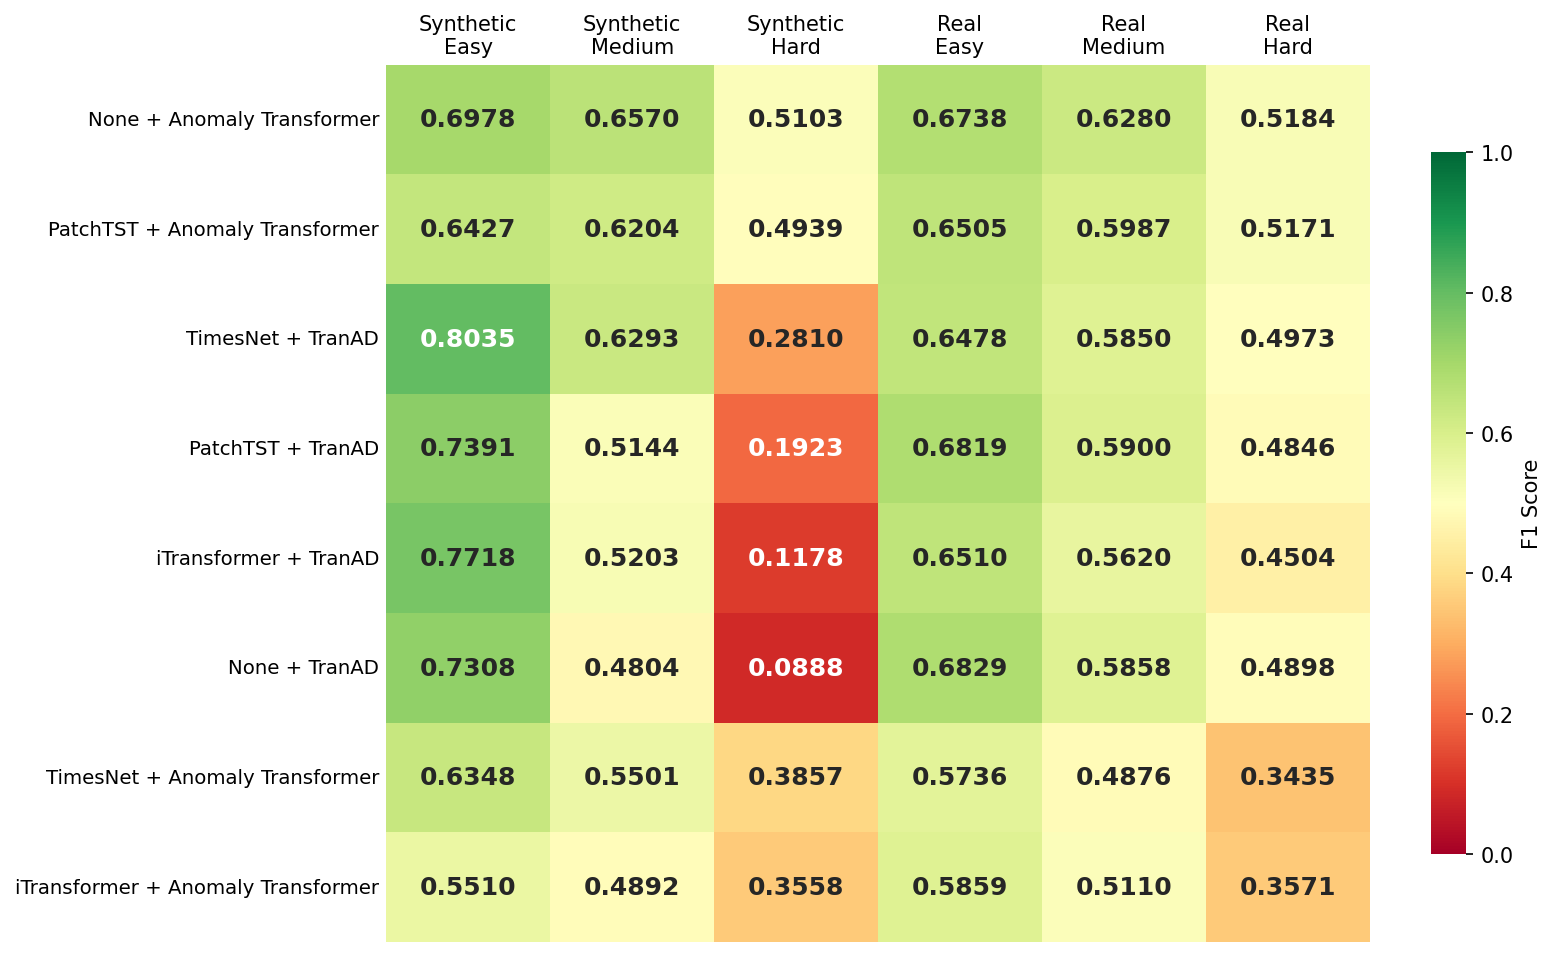
\includegraphics[width=\linewidth]{figures/f1_heatmap.png}
\caption{F1 by substrate and difficulty tier across model variants.}
\label{fig:f1heatmap}
\end{figure}

\begin{table}[H]
\centering
\caption{Pooled recall by anomaly type and difficulty tier (AT-based vs TranAD-based variants).}
\label{tab:recall}
\resizebox{\linewidth}{!}{%
\begin{tabular}{lcccccc}
\toprule
Difficulty & AT Point & TranAD Point & AT Contextual & TranAD Contextual & AT Collective & TranAD Collective \\
\midrule
Easy & 0.374 & 0.923 & 0.836 & 0.893 & 0.353 & 0.390 \\
Medium & 0.341 & 0.747 & 0.753 & 0.664 & 0.291 & 0.166 \\
Hard & 0.304 & 0.464 & 0.468 & 0.265 & 0.256 & 0.193 \\
\bottomrule
\end{tabular}%
}
\end{table}

The AT/TranAD relationship is difficulty-conditional and inverts across anomaly types. For point anomalies, TranAD's advantage compresses sharply with complexity, nearly vanishing under Hard conditions. For contextual anomalies, TranAD leads on Easy but AT pulls ahead on Hard (+0.203), with TranAD's contextual recall dropping 69\% from Easy to Hard against AT's 44\%. For collective anomalies, no variant exceeds 0.457 under any condition, a ceiling consistent with the 96-timestep context-window constraint.

\section{XAI Analysis}

\subsection{Feature Attribution (Integrated Gradients)}

\begin{figure}[t]
\centering
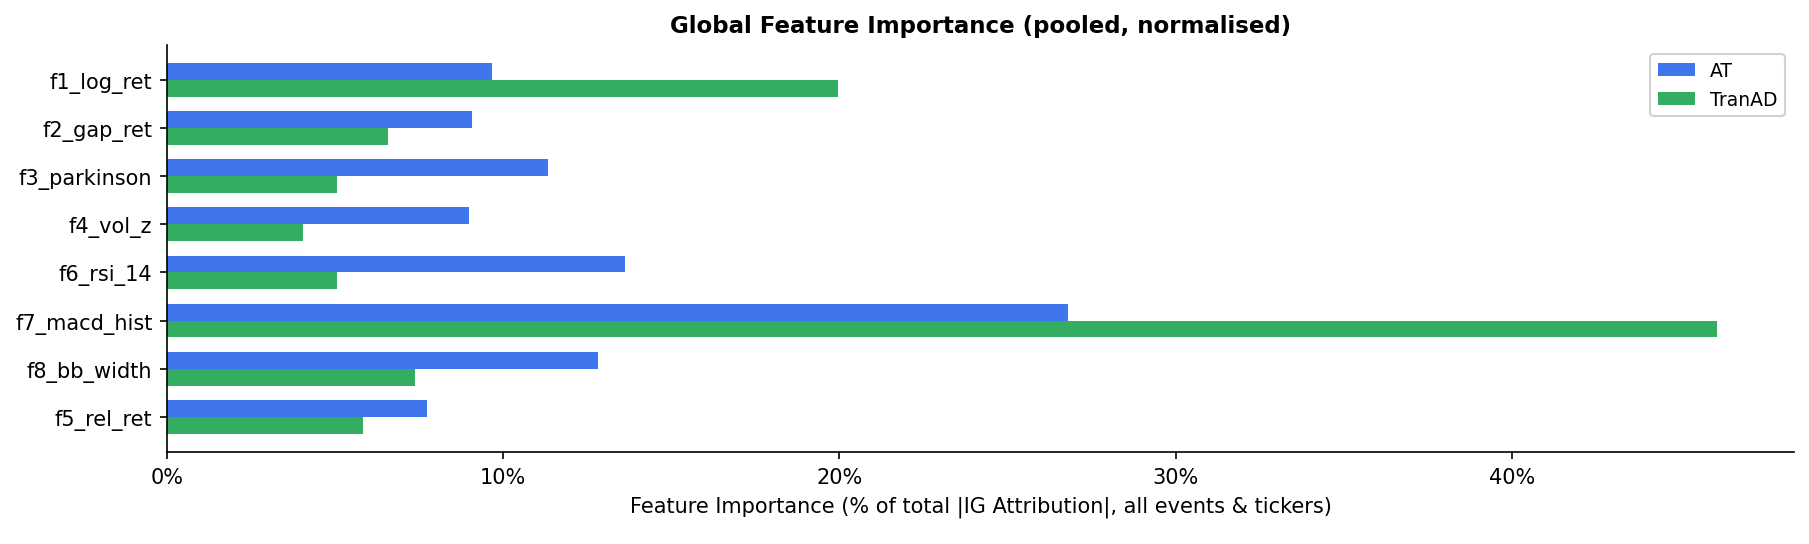
\includegraphics[width=\linewidth]{figures/ig_attribution_global.png}
\caption{Global feature importance (pooled, normalised) across all analyzed events.}
\label{fig:igattribution_global}
\end{figure}

Both detectors anchor on momentum divergence ($f_7$, MACD histogram) for NVDA and TSLA, switching to volatility and gap features for different anomaly types. $f_7$ leads in 14 of 30 AT and 19 of 30 TranAD events, confirming that high-growth anomalies primarily manifest as sustained momentum-regime breaks.

Two systematic deviations are diagnostically significant. During the March 2020 COVID-19 crash, features shift from $f_7$ to volatility indicators, Bollinger Band width ($f_8$) for NVDA and RSI-14 ($f_6$) for TSLA and INTC, identifying the crash as a volatility-regime rather than momentum-divergence event. For INTC events, TranAD produces a profile led by relative return ($f_5$), gap return ($f_2$), and volume ($f_4$), reflecting idiosyncratic earnings shocks rather than sustained breakouts. This demonstrates that TranAD feature leadership implicitly classifies anomalies: $f_5/f_2$-led alerts warrant post-earnings reviews, while $f_7$-led alerts warrant trend-continuation assessments.

AT exhibits gradient saturation failure during large gap-shocks (e.g., INTC Aug 2, 2024; TSLA July 2, 2024): IG attributions collapse to near-zero ($< 10^{-6}$) despite high anomaly scores. TranAD maintains clear attribution for these events, confirming the failure is AT-specific.

\subsection{Temporal Attribution (TimeSHAP)}

TimeSHAP reveals fundamentally different temporal receptive fields. AT exhibits a mean recency concentration of 28\%, while TranAD's 70\% concentration and dominant terminal-state ($t=95$) Shapley values confirm its identity as a terminal detector. Its ``spike-then-suppression'' signature, where $t=95$ values dwarf preceding timesteps, reflects an adversarial stage amplifying terminal deviations against the immediate context.

\begin{figure}[t]
\centering
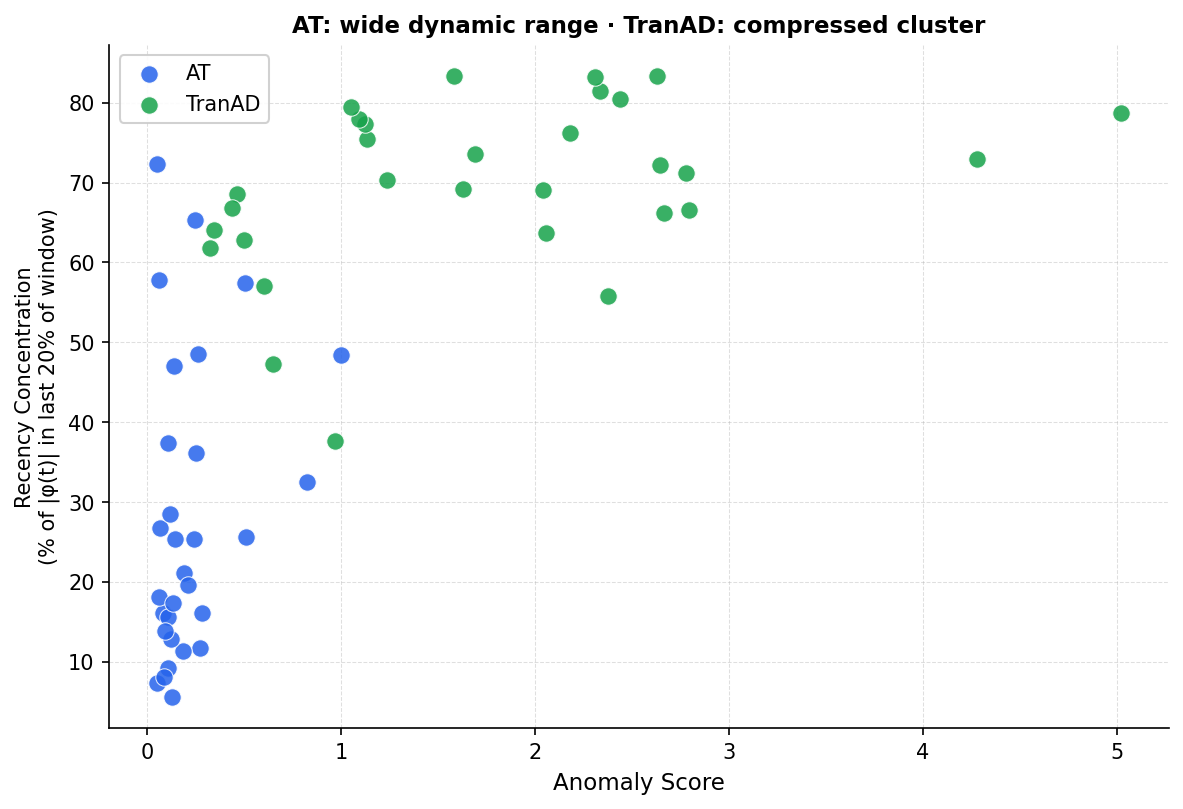
\includegraphics[width=\linewidth]{figures/recency_scatter.png}
\caption{TimeSHAP recency concentration comparison between Anomaly Transformer and TranAD.}
\label{fig:recencyscatter}
\end{figure}

AT's wide recency range (5.6\%--72.3\%) is more diagnostically informative: low concentration indicates integration of multi-week narratives, while high concentration identifies abrupt, self-contained shocks. Recency concentration thus serves as a proxy for distinguishing slow-buildup from sudden-onset events. Conversely, during the 2021 TSLA gamma squeeze, TranAD identified four distinct anomalous sessions with terminal magnitudes tracking the squeeze lifecycle ($+8.00 \rightarrow +7.96 \rightarrow +10.26 \rightarrow +14.80$), while AT collapsed the entire two-week period into a single flagged date.

\subsection{Event Attribution (LLM-Ranked News Retrieval)}

\textbf{Strong corroboration - NVDA August 5, 2024 (AT: 0.827):} The LLM identifies three concurrent catalysts, Blackwell design flaws, a DOJ probe, and a Japan-led market rout, correctly weighting the Blackwell delay ($9/10$). AT's near-terminal Shapley ($t = 91$) and 32.5\% recency concentration indicate a sudden shock, while $f_7$ leadership confirms a momentum-reversal event.

\textbf{Partial corroboration - INTC August 2, 2024 (TranAD: 1.628):} The LLM correctly attributes the crash to Intel's Q2 earnings, dividend cuts, and a 15,000-person layoff ($10/10$). However, IG reveals AT's gradient saturation failure for this same event: news attribution remains clear while feature attribution collapses, underscoring the value of joint tri-layer analysis.

\textbf{Temporal ambiguity - NVDA January 27, 2025 (AT: 0.510):} The LLM identifies the DeepSeek release behind a \$593 billion market cap decline. AT's distributed TimeSHAP profile (recency 25.6\%, dominant $t = 55$) suggests the model integrated accumulated AI-capex narrative tension alongside the immediate shock, the model detected a "prepared fault line", not just the "earthquake".

\section{Discussion and Limitations}

\subsection{Discussion}

The XAI analysis makes detection complementarity mechanistically explicit: TranAD's terminal-state focus and high point-anomaly recall suit sharp, sudden shocks, while AT's distributed temporal attention and superior contextual recall suit sustained regime deviations. All three XAI layers provide non-redundant information, the INTC August 2024 case demonstrates that news attribution can be maximally informative while IG simultaneously fails. In practice, TranAD is preferred for earnings surveillance given its sensitivity to gap shocks ($f_2$) and idiosyncratic relative return ($f_5$), while AT is the stronger choice for regime monitoring requiring multi-week narrative integration. In a production system, the two are best deployed in parallel, with alert routing determined by the leading feature and recency concentration of each detection.

\subsection{Limitations}

\textbf{Methodological and Evaluation:} The most significant limitation is the Point Adjustment protocol, which inflates recall for contextual and collective anomaly types with 10--20 day windows~\cite{ref14,ref4}; reported values should be treated as upper bounds. The absence of non-deep-learning baselines (e.g., Isolation Forest, One-Class SVM) leaves absolute performance unanchored against classical methods, the most significant gap for future work. All models were trained on US equities and may not generalise to FX, cryptocurrency, or fixed income markets.

\textbf{Interpretability:} IG attributions use a zero feature vector baseline with no direct economic interpretation; replacing this with a feature-wise mean of normal periods is the highest-leverage XAI improvement. Partial gradient detachment in AT's association discrepancy path produces the saturation failure observed on the INTC August 2024 event. TimeSHAP estimates carry non-negligible Monte Carlo variance at $n = 50$ permutations, and the LLM news layer's 24-hour lookahead window makes it unsuitable for real-time deployment.

\textbf{Benchmark and Data:} The Easy/Medium/Hard injection tiers are artificial constructs whose correspondence to real anomaly distributions is unverified. The collective recall ceiling (no model exceeds 0.457) is consistent with the 96-timestep context-window constraint and should not be treated as an architectural differentiator until tested under extended windows. The 8-feature panel omits options-market signals (implied volatility, put/call ratios) and order-flow features, limiting attribution depth for derivatives-driven events such as the TSLA gamma squeeze.

\section{Conclusion}

This paper presented an anomaly detection and attribution framework for financial time series, evaluating a modular Embedder $\rightarrow$ Detector architecture across a dual-substrate benchmark with a three-layer interpretability stack. Embedder benefit is architecture-conditional: AT performs best without an upstream embedder, while TimesNet provides selective gains for TranAD. The two detectors exhibit complementary profiles, TranAD excels at point anomaly recall but collapses on contextual anomalies and incurs a synthetic substrate penalty, while AT maintains robust contextual recall that widens with difficulty.

The XAI analysis grounds these differences mechanistically: TranAD's 70\% terminal-timestep attribution mass identifies it as a threshold detector suited to sharp shocks, while AT's recency concentration (5.6\%--72.3\%) functions as an implicit anomaly-structure classifier. MACD histogram dominance across both models confirms momentum divergence as the primary signal for growth-oriented tickers, while the feature shift for INTC events demonstrates that the attribution layer can classify anomaly type and enable targeted alert routing. Future work should pursue PA-free evaluation, extended context windows to probe the collective recall ceiling, non-DL baseline comparisons, and enrichment with options-market and order-flow features toward a fully multimodal anomaly explanation system.

\clearpage
\begin{thebibliography}{99}

\bibitem{ref1}
Bento, J., Saleiro, P., Cruz, A.F., Figueiredo, M.A.T., Bizarro, P.:
TimeSHAP: Explaining Recurrent Models through Sequence Perturbations.
In: Proc. 27th ACM SIGKDD Conference on Knowledge Discovery and Data Mining, pp. 2565--2573.
ACM, New York (2021)

\bibitem{ref2}
Cao, L., Yang, D., Wang, Q., Yu, Y., Wang, J., Rundensteiner, E.A.:
Detecting Financial Fraud Using Machine Learning: Winning the War Against Imbalanced Data.
In: Proc. ACM International Conference on AI in Finance (ICAIF).
ACM, New York (2019)

\bibitem{ref3}
Engle, R.F.:
Autoregressive Conditional Heteroscedasticity with Estimates of the Variance of United Kingdom Inflation.
Econometrica \textbf{50}(4), 987--1007 (1982)

\bibitem{ref4}
Liu, S., Paparrizos, J.:
Elephant in the Room: Towards a Reliable Time-Series Anomaly Detection Benchmark.
In: Advances in Neural Information Processing Systems, vol.~37.
Curran Associates (2024)

\bibitem{ref5}
Liu, Y., Hu, T., Zhang, H., Wu, H., Wang, S., Ma, L., Long, M.:
iTransformer: Inverted Transformers Are Effective for Time Series Forecasting.
In: Proc. 12th International Conference on Learning Representations (ICLR 2024) (2024)

\bibitem{ref7}
Malhotra, P., Ramakrishnan, A., Anand, G., Vig, L., Agarwal, P., Shroff, G.:
LSTM-based Encoder-Decoder for Multi-sensor Anomaly Detection.
In: ICML 2016 Anomaly Detection Workshop (2016)

\bibitem{ref8}
McNeil, A.J., Frey, R.:
Estimation of Tail-Related Risk Measures for Heteroscedastic Financial Time Series.
J. Empirical Finance \textbf{7}(3--4), 271--300 (2000)

\bibitem{ref9}
Nie, Y., Nguyen, N.H., Sinthong, P., Kalagnanam, J.:
A Time Series is Worth 64 Words: Long-term Forecasting with Transformers.
In: Proc. 11th International Conference on Learning Representations (ICLR 2023) (2023)

\bibitem{ref10}
Park, D., Kim, Y., Ha, I., Oh, S.:
A Multimodal Anomaly Detector for Robot-Assisted Feeding Using an LSTM-based Variational Autoencoder.
IEEE Robot. Autom. Lett. \textbf{3}(3), 1544--1551 (2018)

\bibitem{ref11}
Sundararajan, M., Taly, A., Yan, Q.:
Axiomatic Attribution for Deep Networks.
In: Proc. 34th International Conference on Machine Learning.
PMLR \textbf{70}, 3319--3328 (2017)

\bibitem{ref12}
Tuli, S., Casale, G., Jennings, N.R.:
TranAD: Deep Transformer Networks for Anomaly Detection in Multivariate Time Series Data.
Proc. VLDB Endow. \textbf{15}(6), 1201--1214 (2022)

\bibitem{ref13}
Wu, H., Hu, T., Liu, Y., Zhou, H., Wang, J., Long, M.:
TimesNet: Temporal 2D-Variation Modeling for General Time Series Analysis.
In: Proc. 11th International Conference on Learning Representations (ICLR 2023) (2023)

\bibitem{ref14}
Wu, R., Keogh, E.:
Current Time Series Anomaly Detection Benchmarks are Flawed and are Creating the Illusion of Progress.
IEEE Trans. Knowl. Data Eng. \textbf{35}(3), 2421--2429 (2023)

\bibitem{ref15}
Xu, J., Wu, H., Wang, J., Long, M.:
Anomaly Transformer: Time Series Anomaly Detection with Association Discrepancy.
In: Proc. 10th International Conference on Learning Representations (ICLR 2022) (2022)

\bibitem{ref16}
Zhou, H., Zhang, S., Peng, J., Zhang, S., Li, J., Xiong, H., Zhang, W.:
Informer: Beyond Efficient Transformer for Long Sequence Time-Series Forecasting.
In: Proc. 35th AAAI Conference on Artificial Intelligence, vol.~35, pp. 11106--11115.
AAAI Press (2021)

\bibitem{ref17}
Kroeger, N., Ley, D., Jacob, M., Bhatt, U., Adebayo, J.:
Are Large Language Models Post Hoc Explainers?
NeurIPS 2023 Workshop on Robustness of Few/Zero-shot Learning in Foundation Models.
arXiv:2310.05797 (2023)

\bibitem{ref18}
Google:
Gemini 3.1 Flash-Lite Model Documentation.
Google Cloud Vertex AI, \url{https://cloud.google.com/vertex-ai/generative-ai/docs/models/gemini/3-1-flash-lite} (2026)

\bibitem{ref19}
Ahmed, M., Mahmood, A.N., Hu, J.:
A Survey of Network Anomaly Detection Techniques.
J. Netw. Comput. Appl. \textbf{60}, 19--31 (2016)

\end{thebibliography}

\clearpage
\appendix
\renewcommand{\thefigure}{A\arabic{figure}}
\setcounter{figure}{0}
\section{Analysis Figures}

Figures A1--A6 present the full three-panel analysis plots (anomaly score, log return deviation, and price reconstruction with anomaly spans) for each ticker-model combination. These figures illustrate the qualitative behavioral differences between the Anomaly Transformer and TranAD discussed in Sects.~4 and~5.

\begin{figure}[H]
\centering
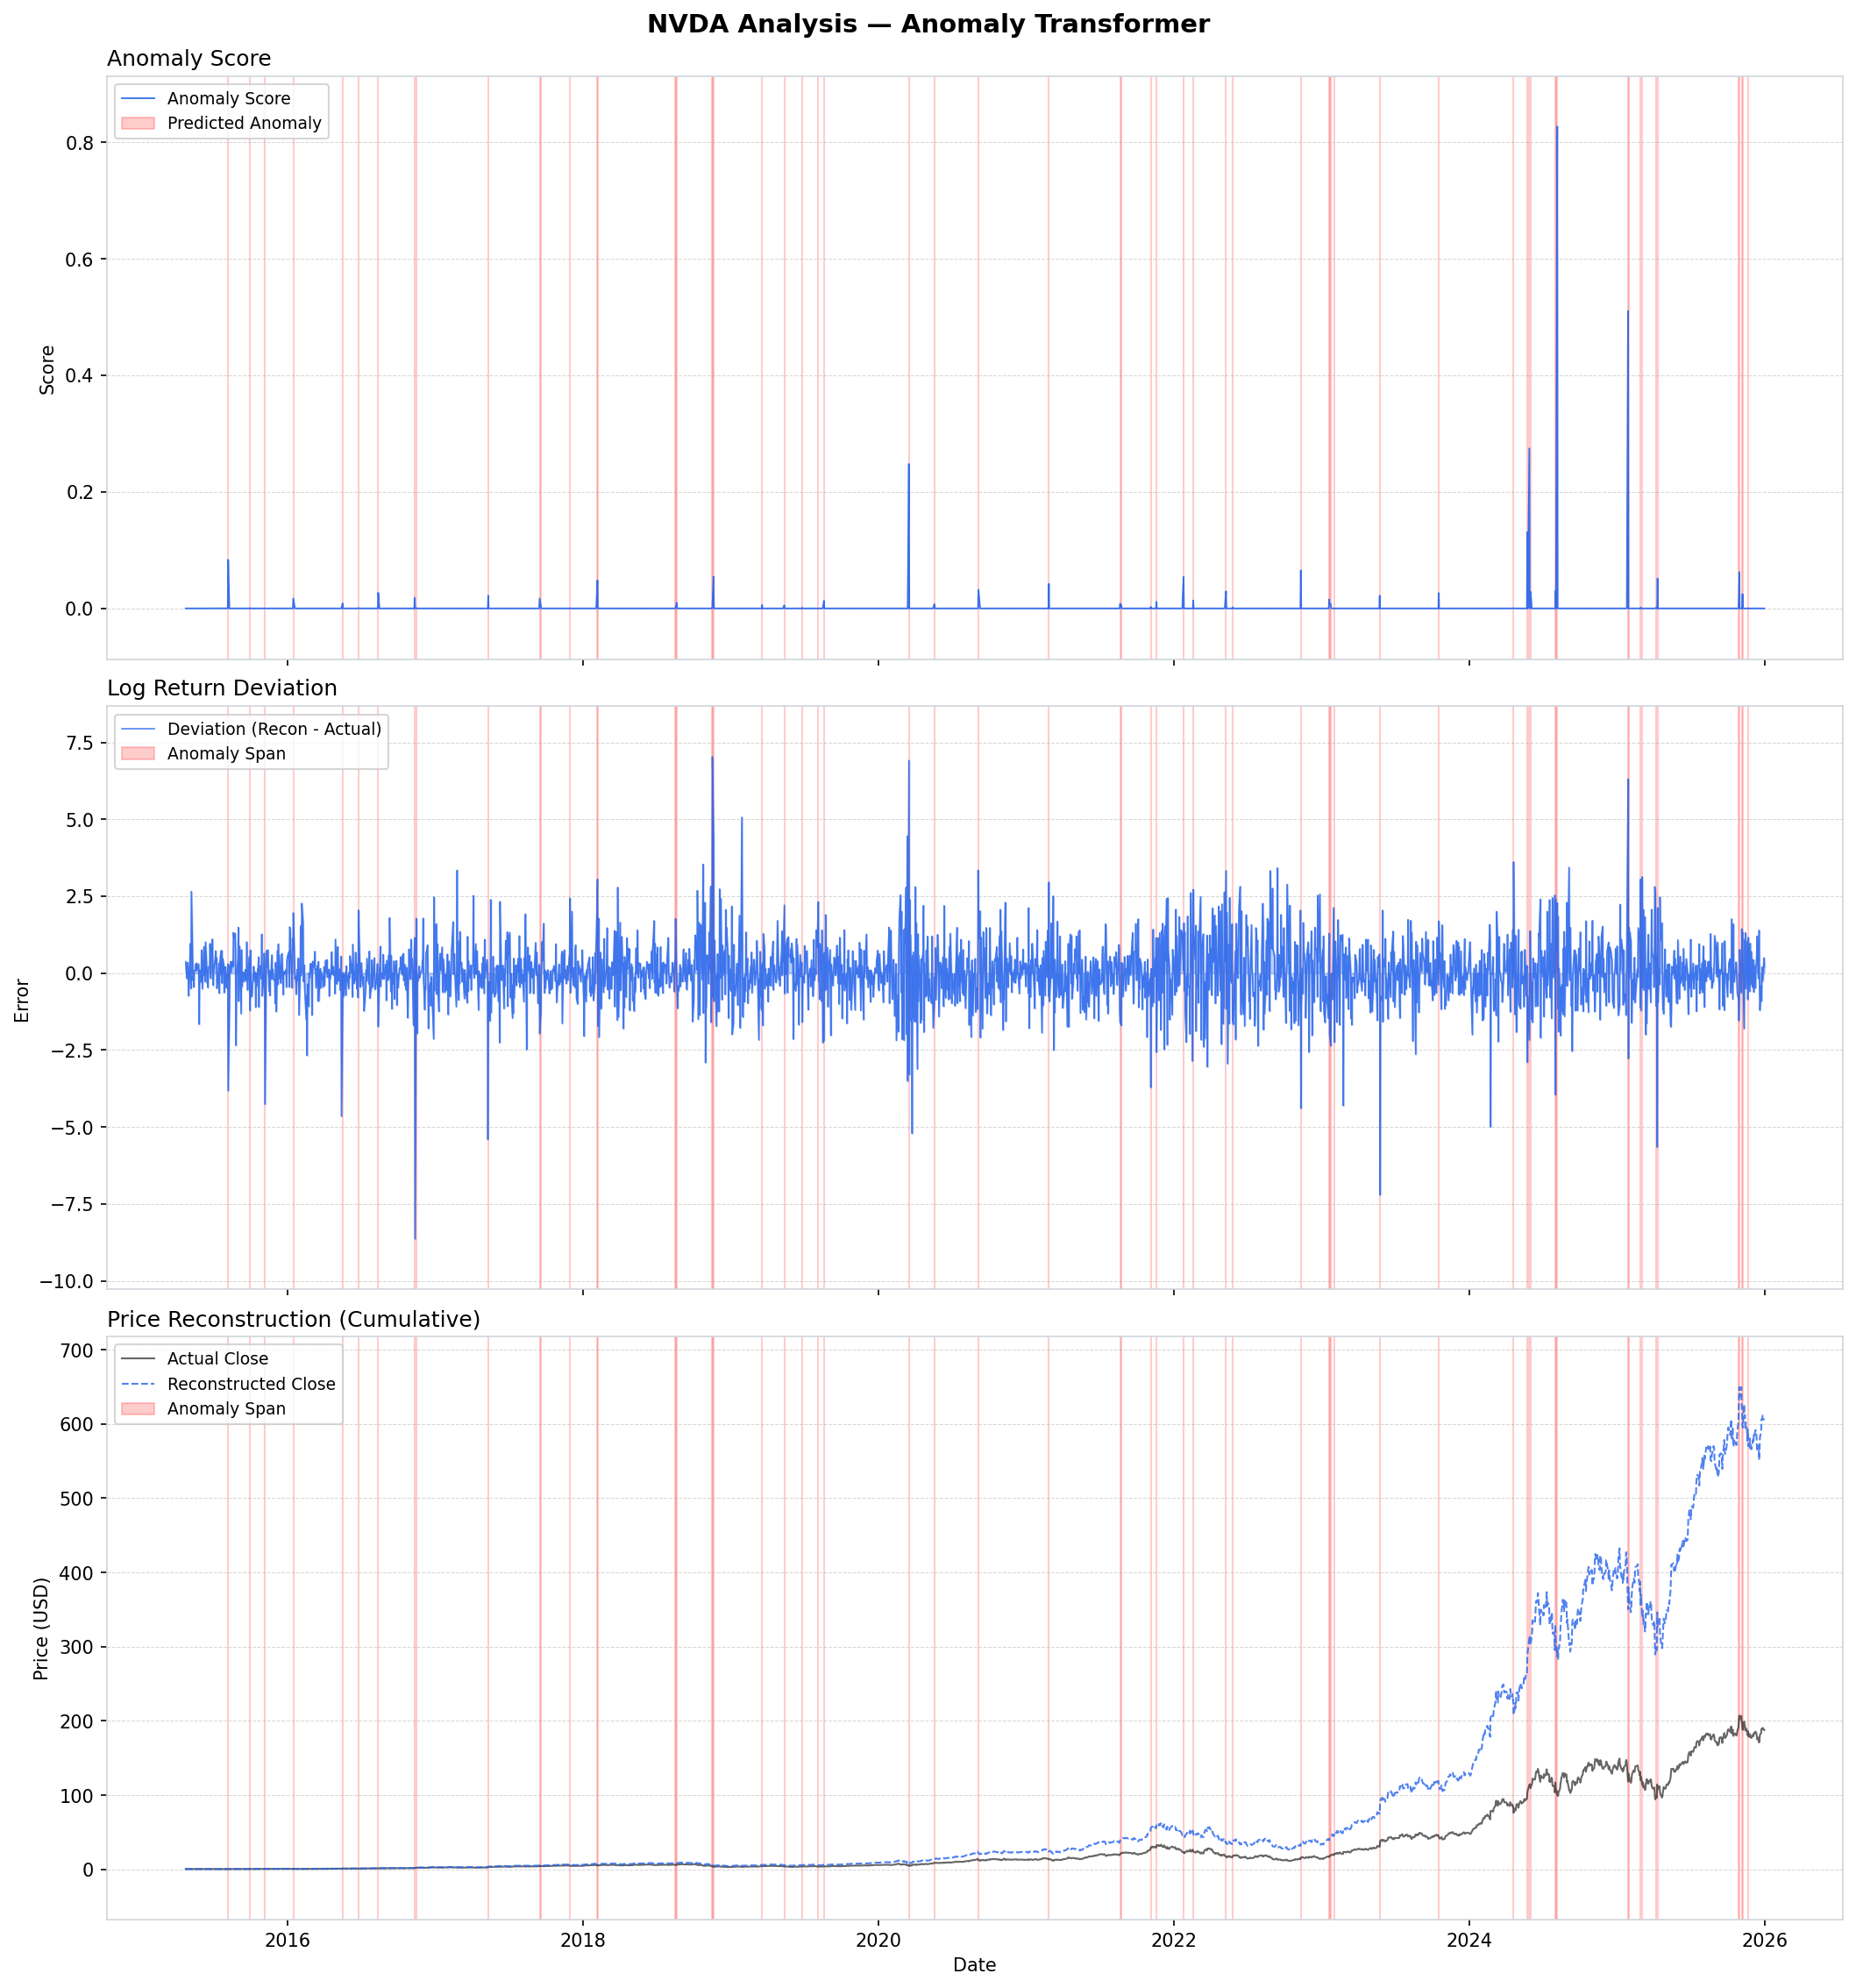
\includegraphics[width=\linewidth]{figures/figure_A1.png}
\caption{NVDA analysis under the Anomaly Transformer. Top: anomaly score series with flagged regions. Middle: log return deviation (reconstructed - actual). Bottom: actual vs reconstructed close price with anomaly spans. Note the sparse, event-driven flagging pattern and the score spike at August 2024 (Blackwell delays + DOJ probe) and January 2025 (DeepSeek).}
\label{fig:A1}
\end{figure}

\begin{figure}[H]
\centering
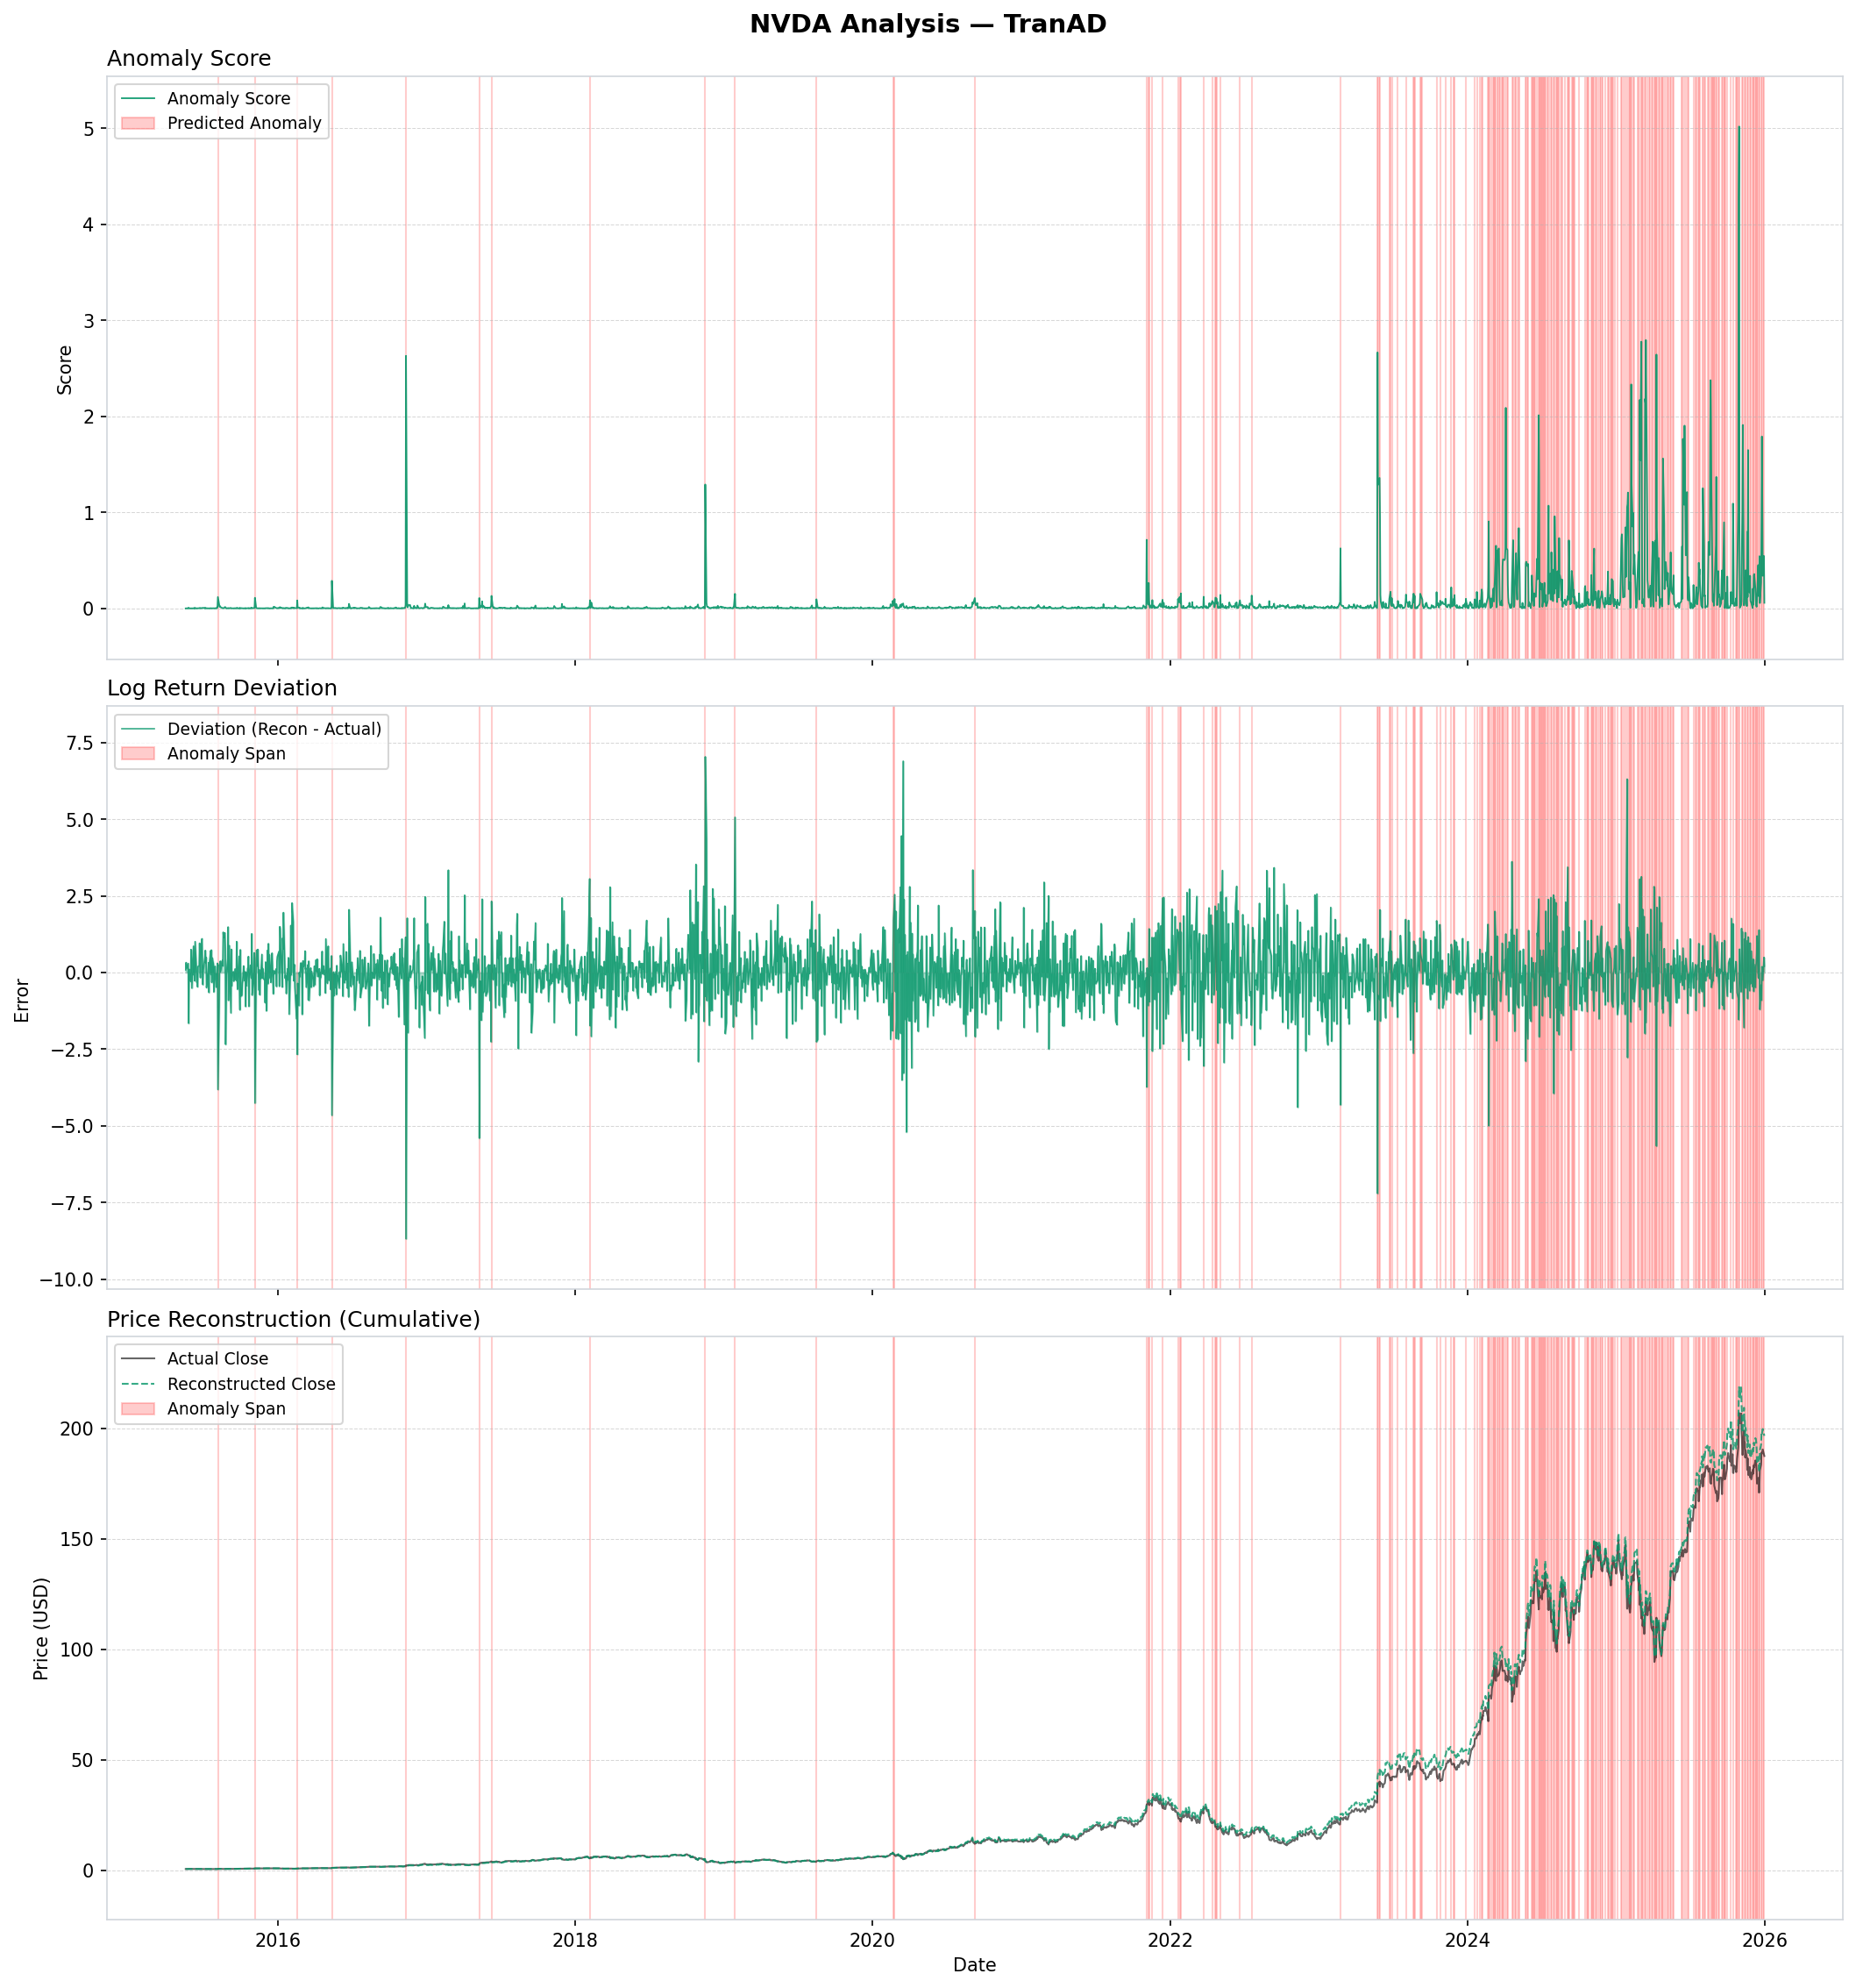
\includegraphics[width=\linewidth]{figures/figure_A2.png}
\caption{NVDA analysis under TranAD. Note the dense flagging beginning in 2023 during NVDA's AI-driven hypergrowth regime, reflecting a distribution shift between the broad training distribution and regime-change ticker behaviour rather than an architectural failure.}
\label{fig:A2}
\end{figure}

\begin{figure}[H]
\centering
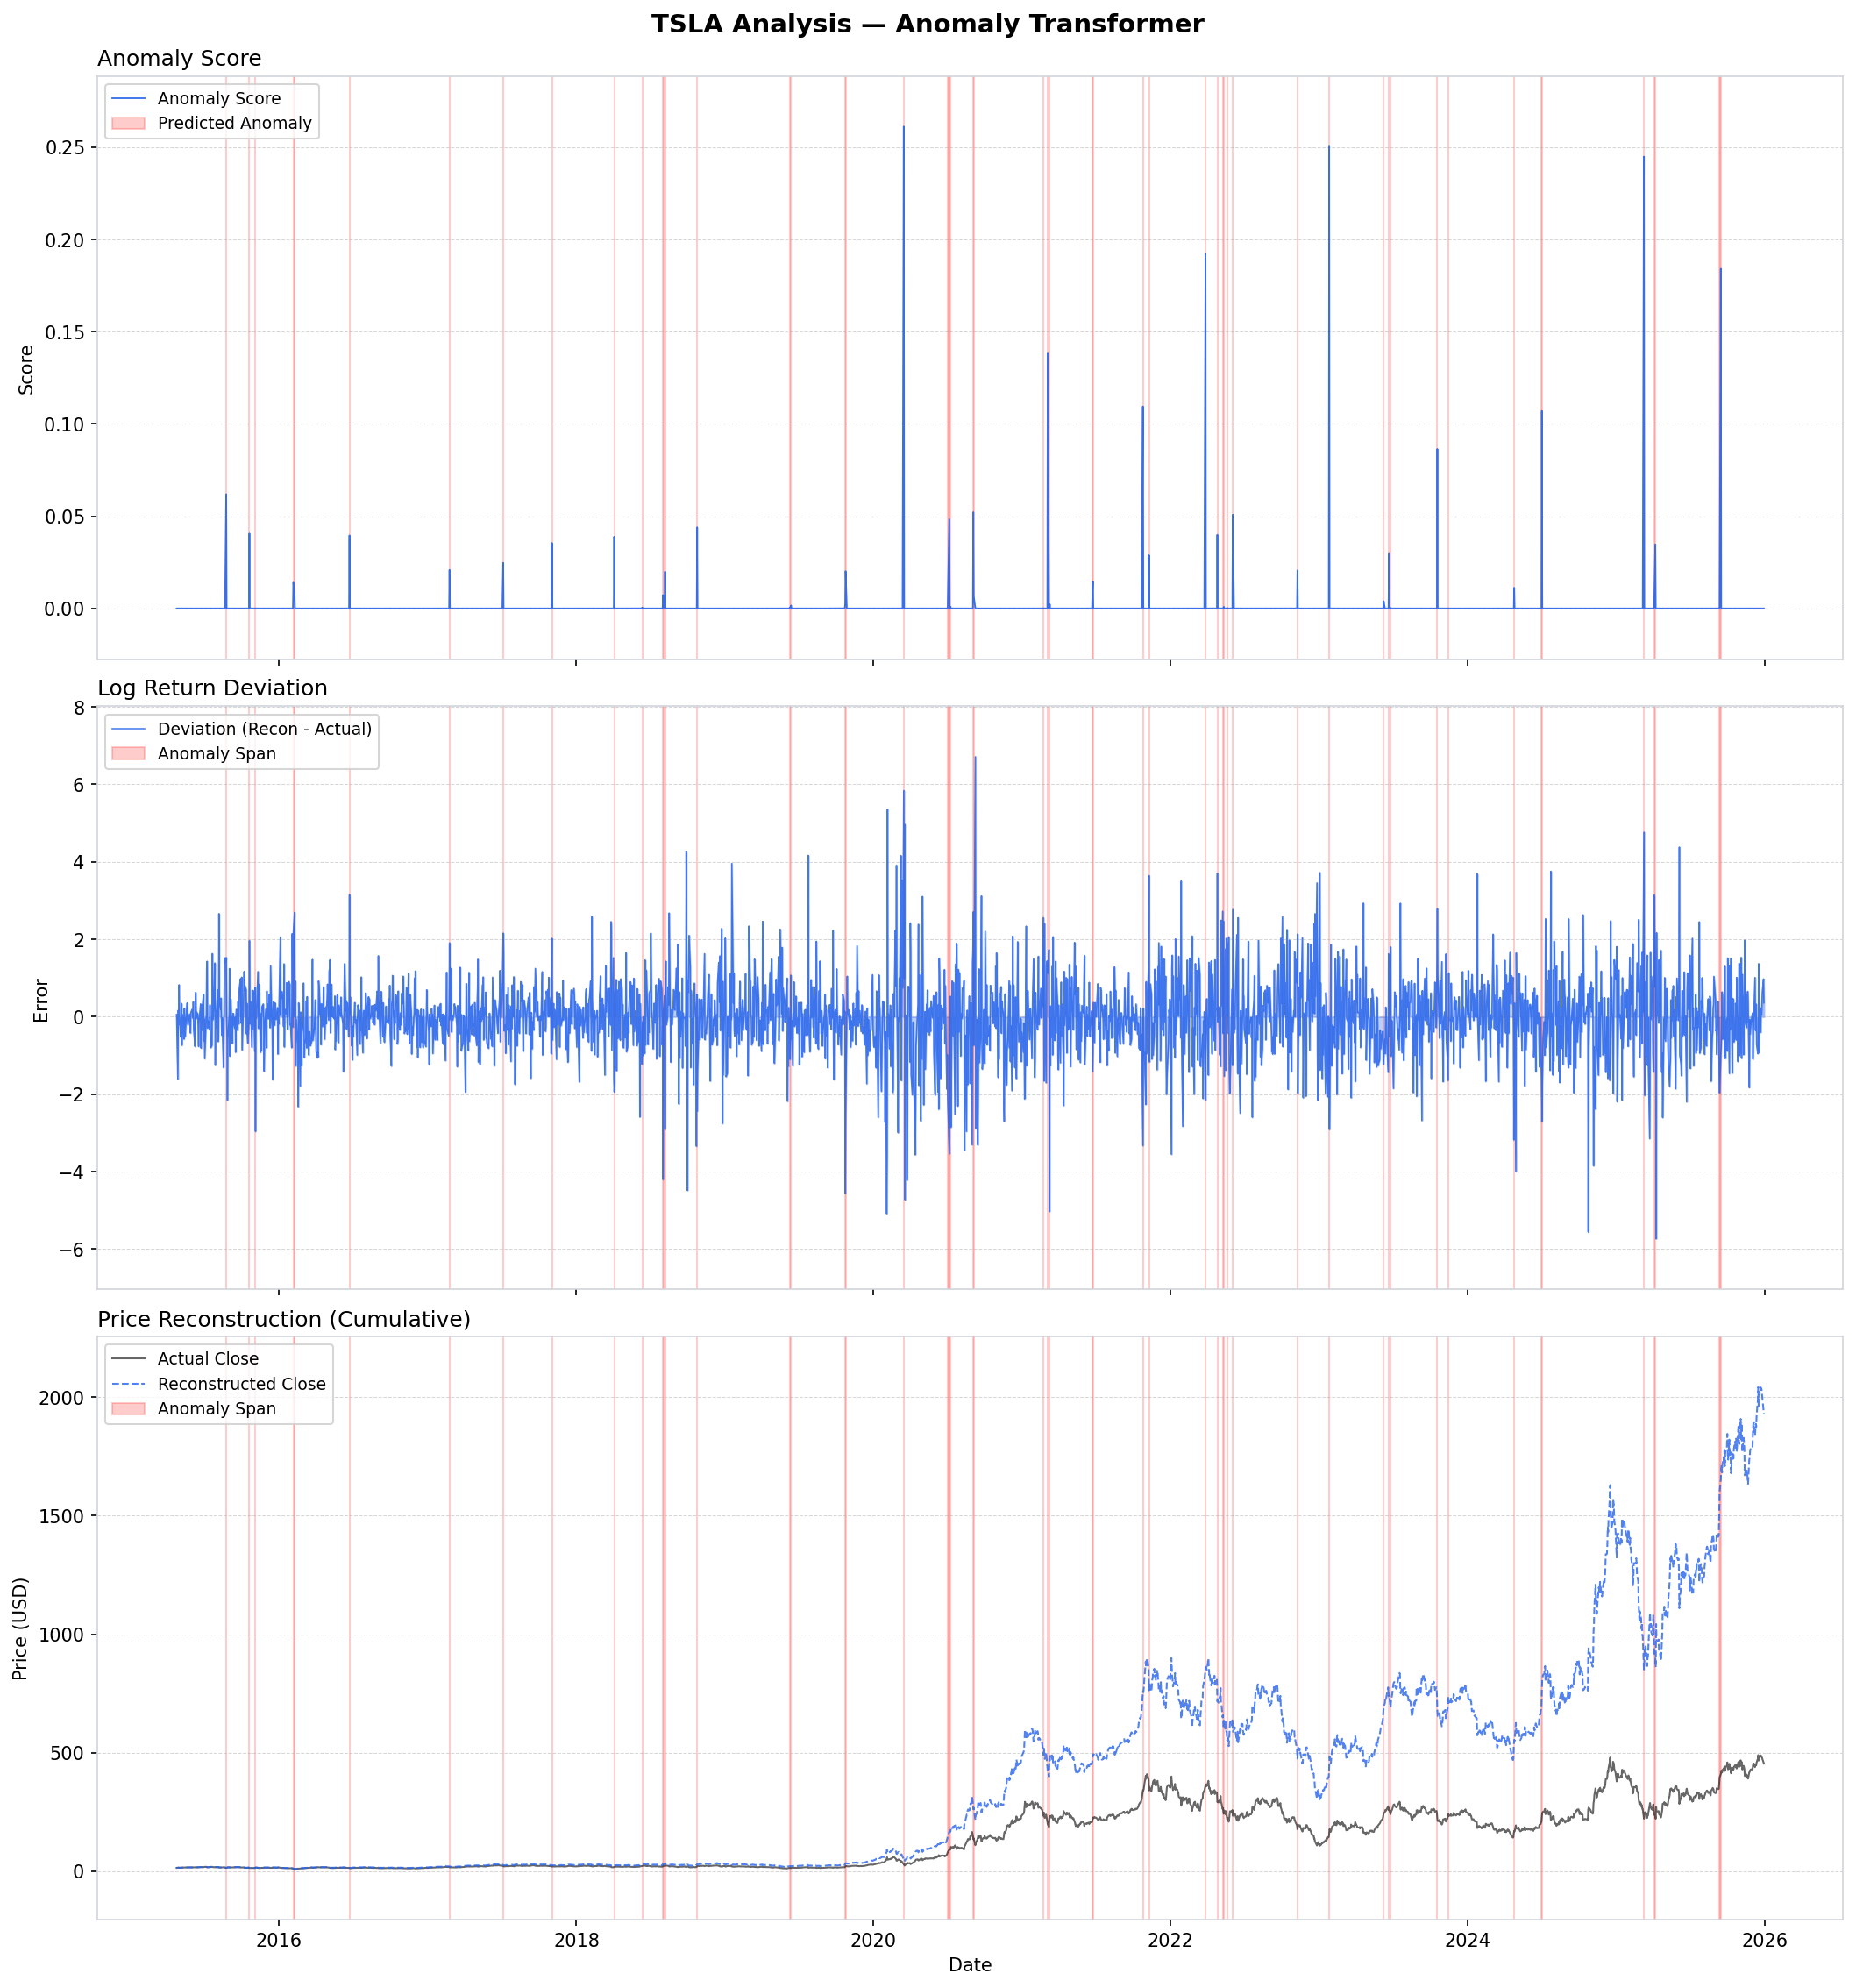
\includegraphics[width=\linewidth]{figures/figure_A3.png}
\caption{TSLA analysis under the Anomaly Transformer. Sparse discrete score spikes correspond to identifiable events: COVID crash (March 2020), Hertz deal period (October--November 2021), and the March 2025 brand crisis event.}
\label{fig:A3}
\end{figure}

\begin{figure}[H]
\centering
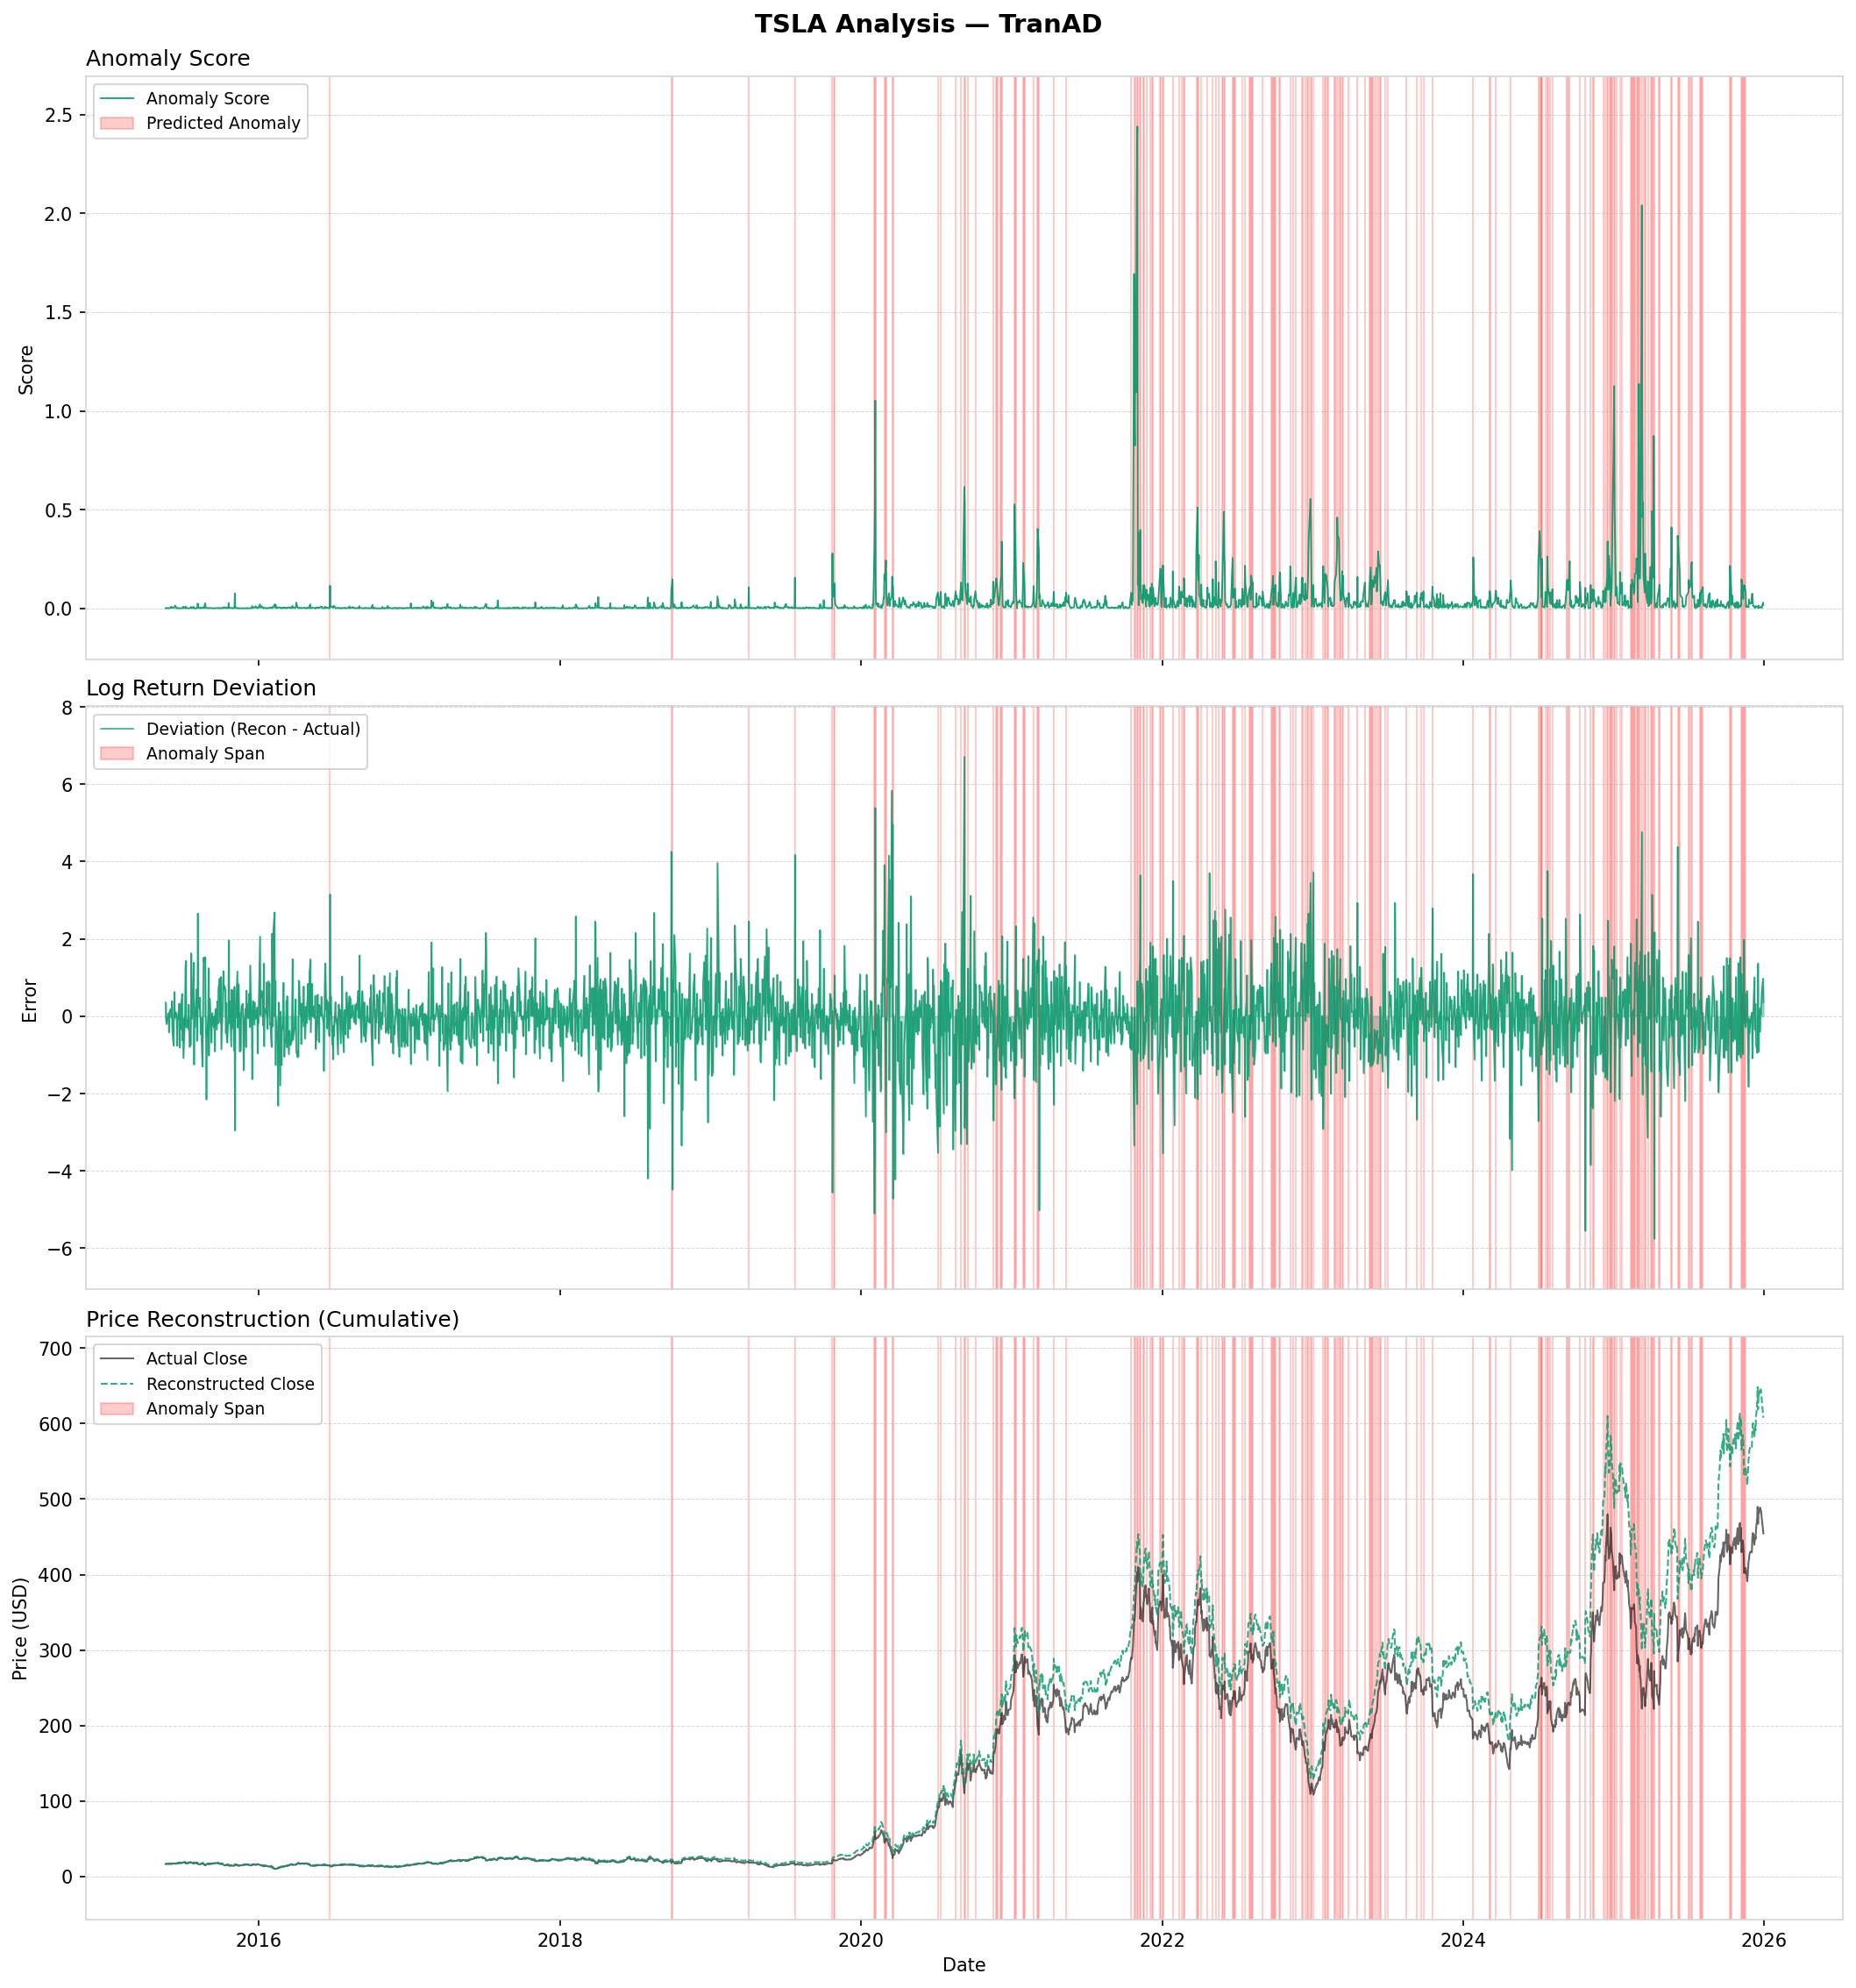
\includegraphics[width=\linewidth]{figures/figure_A4.png}
\caption{TSLA analysis under TranAD. Broad flagging from 2021 onward corresponds to TSLA's elevated volatility regime following the Hertz deal and post-2020 retail-driven momentum period.}
\label{fig:A4}
\end{figure}

\begin{figure}[H]
\centering
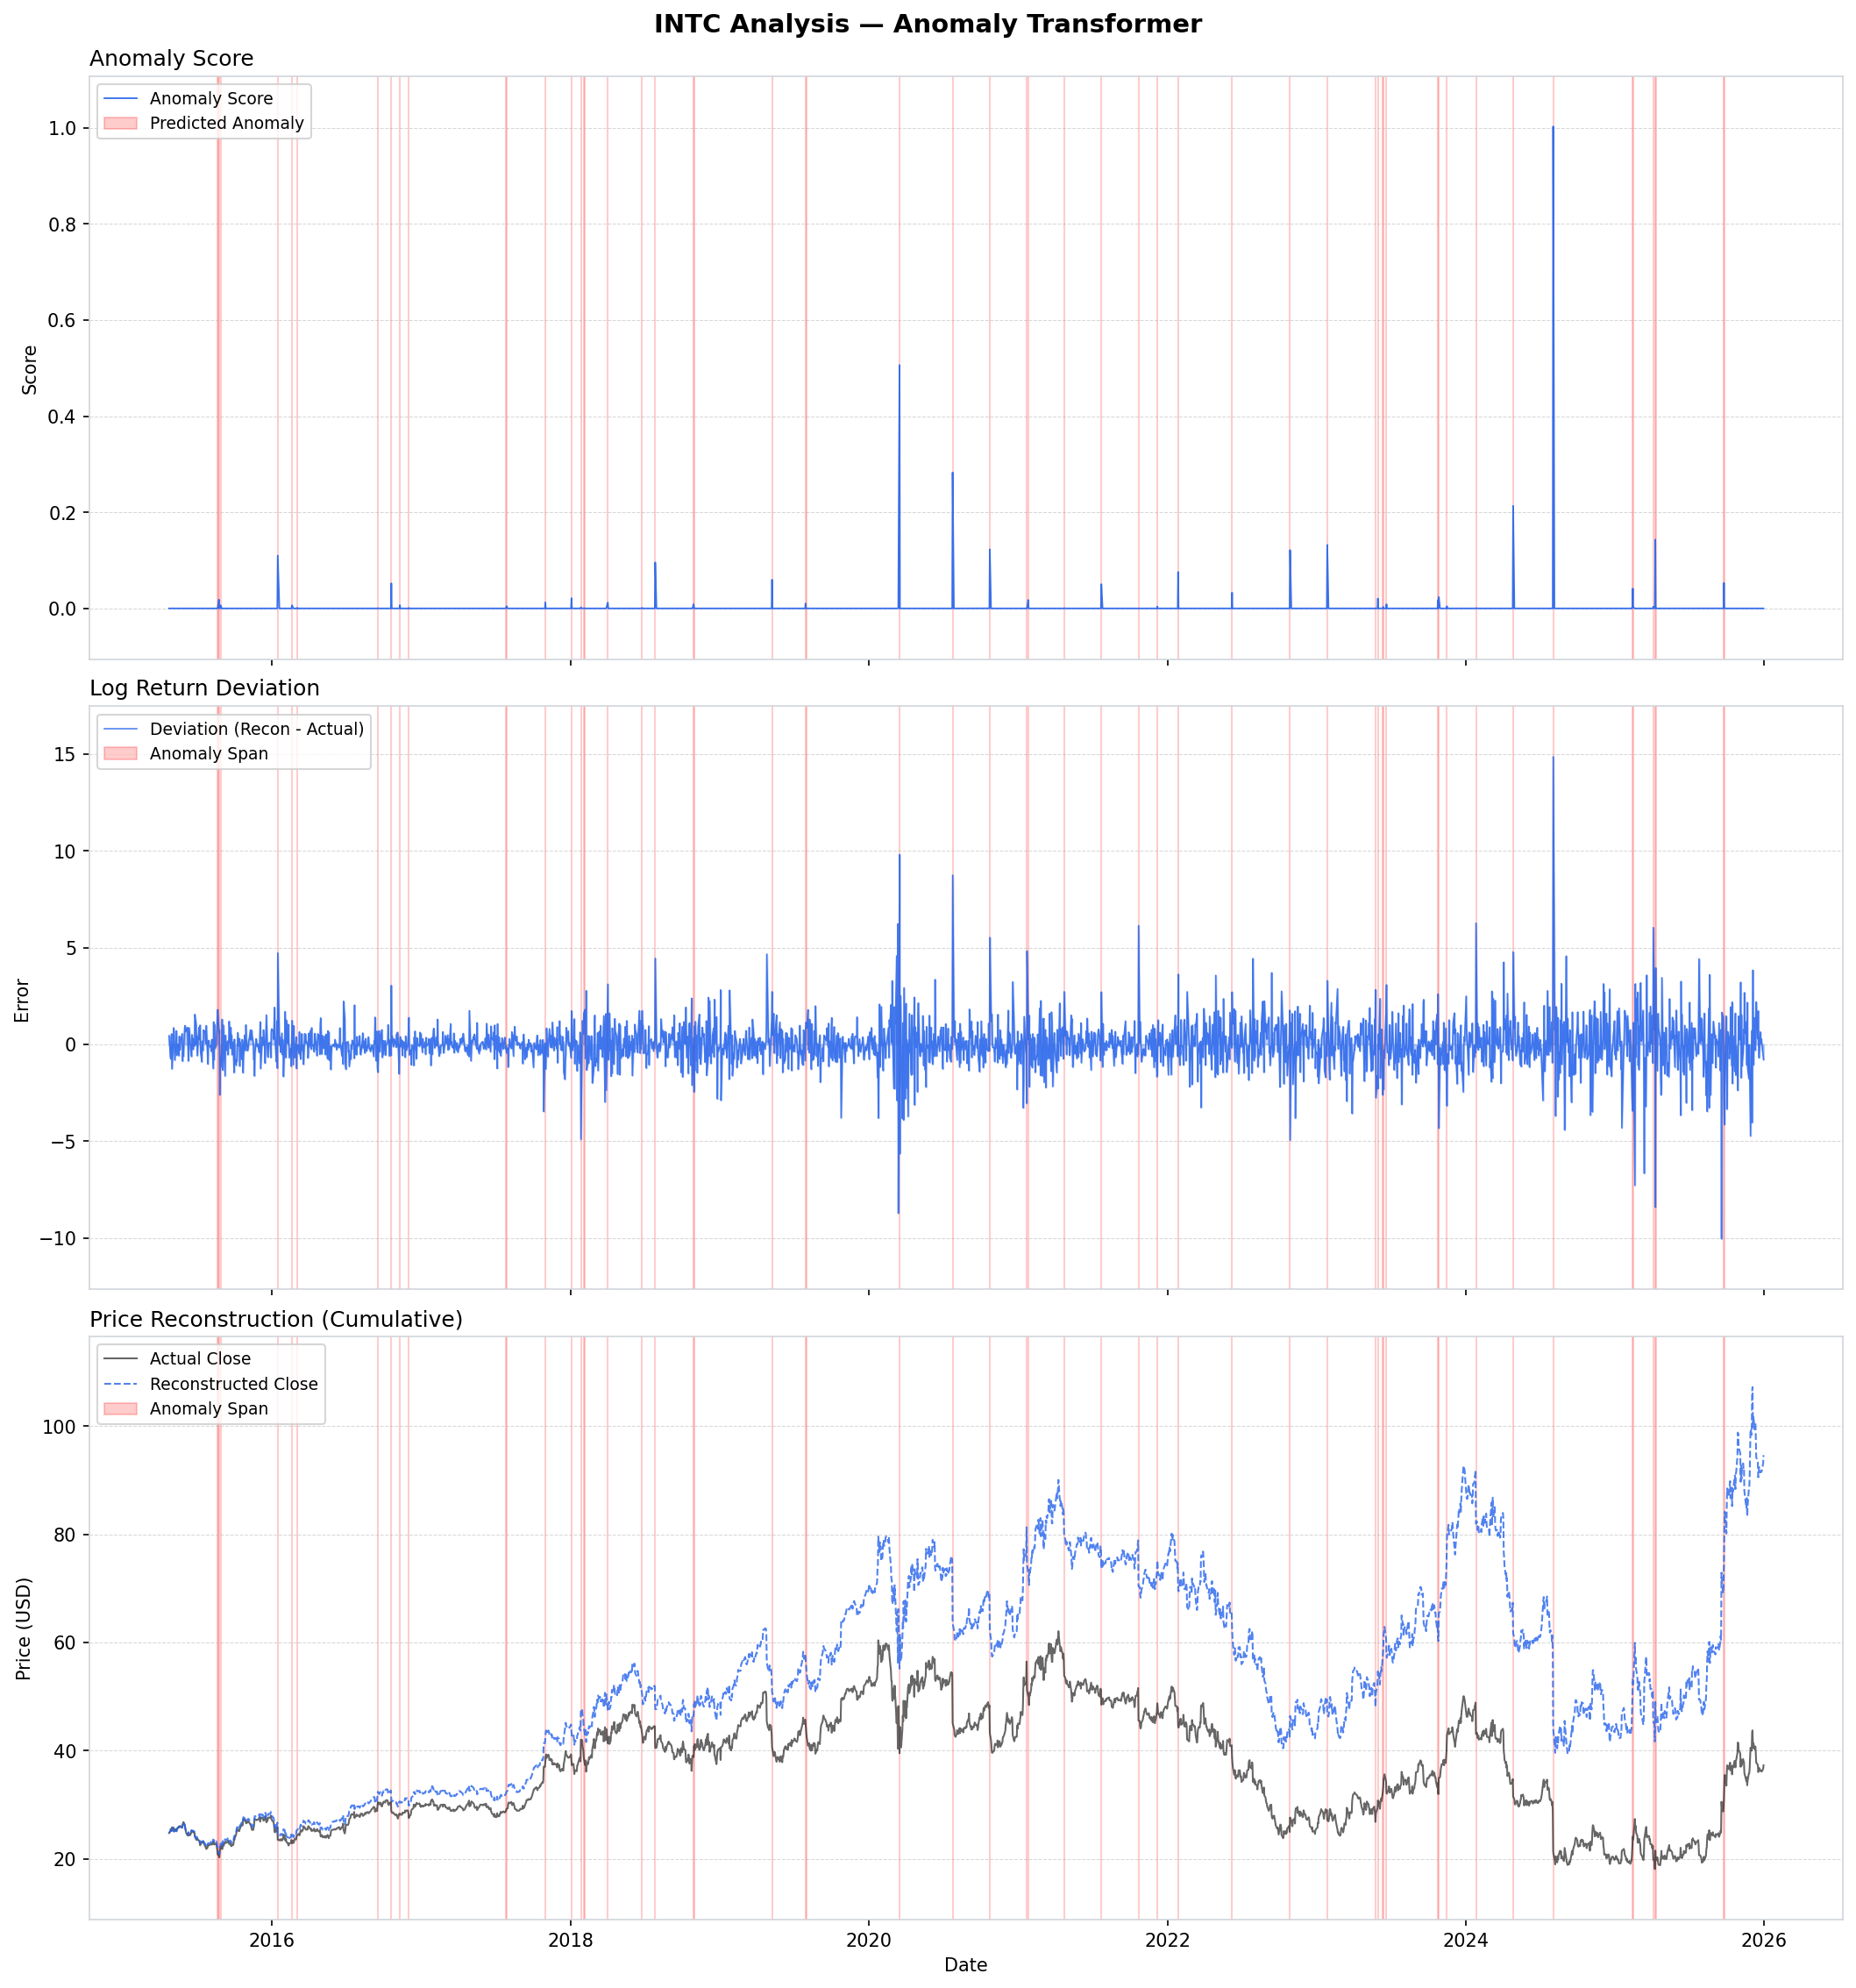
\includegraphics[width=\linewidth]{figures/figure_A5.png}
\caption{INTC analysis under the Anomaly Transformer. The highest-scored event (August 2024, score = 1.003) corresponds to Intel's catastrophic Q2 earnings; this event also exhibits the gradient saturation failure discussed in Sect.~5.1.}
\label{fig:A5}
\end{figure}

\begin{figure}[H]
\centering
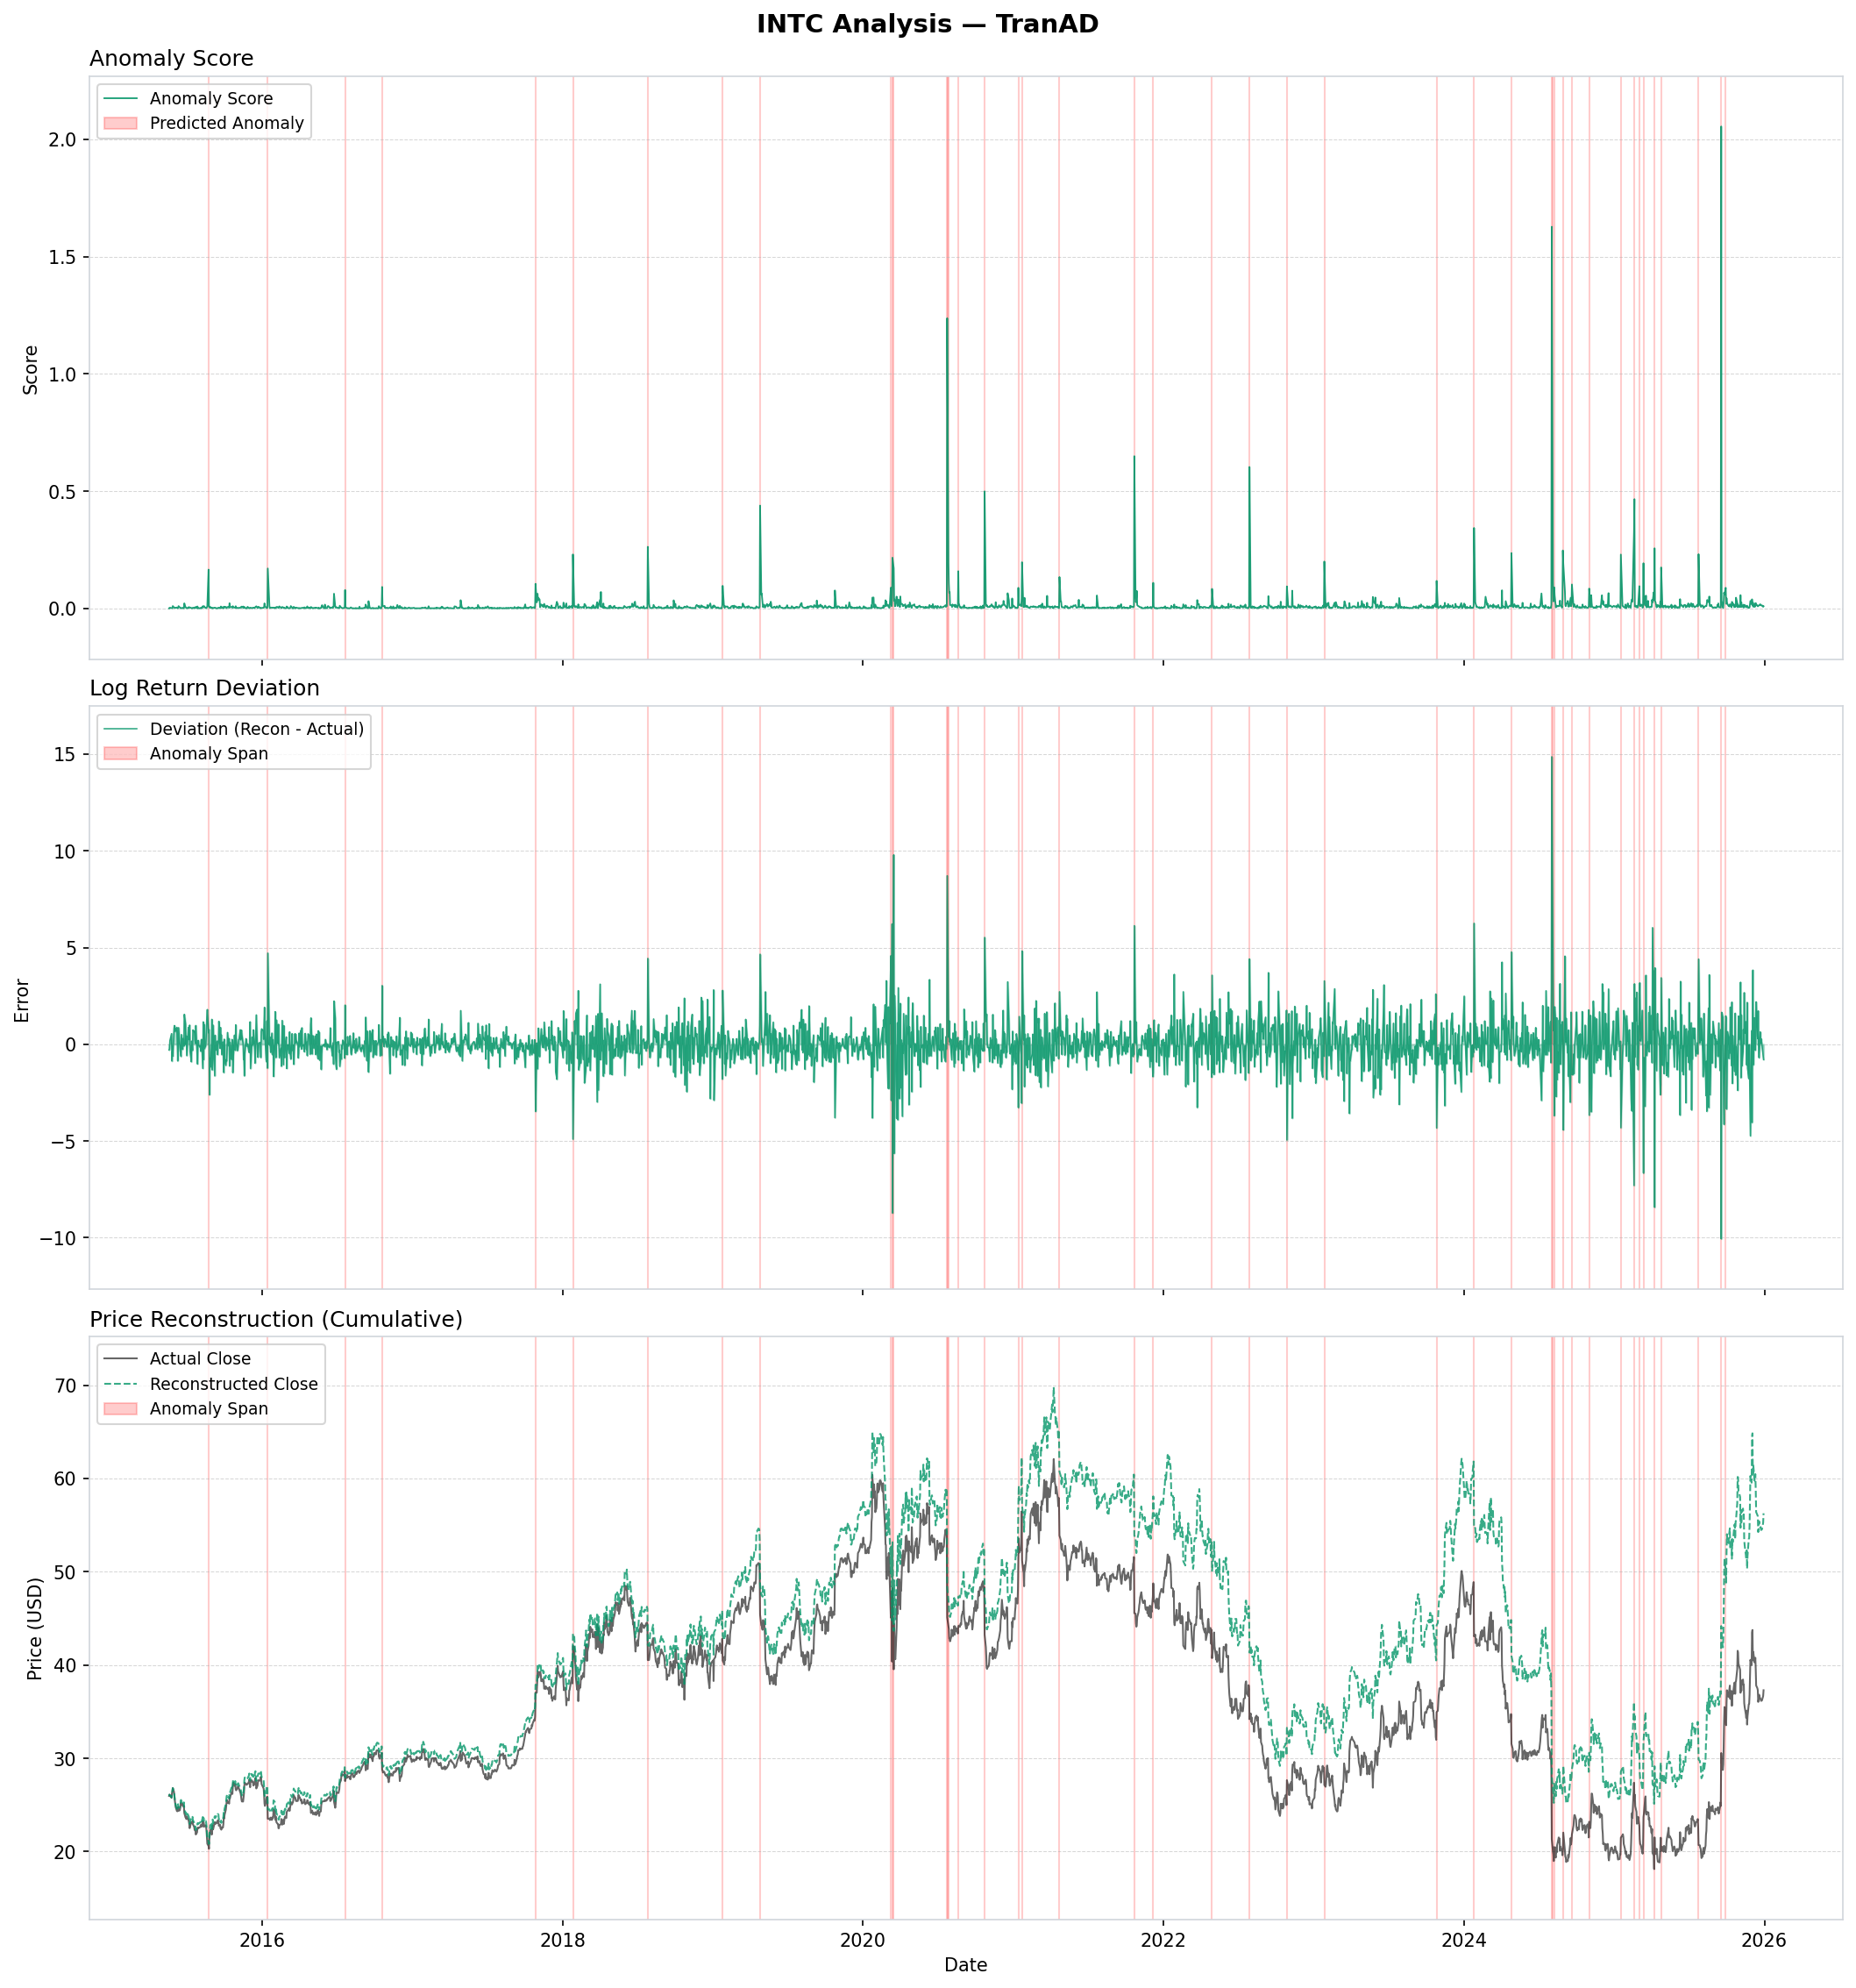
\includegraphics[width=\linewidth]{figures/figure_A6.png}
\caption{INTC analysis under TranAD. Unlike NVDA and TSLA, INTC shows more measured flagging without a broad regime-change over-flagging pattern, consistent with Intel's gradual fundamental decline rather than explosive upward growth.}
\label{fig:A6}
\end{figure}

\section{Pipeline Details}
\label{app:methodology}

\subsection*{Feature Definitions}

The eight engineered features are defined as follows:
\begin{itemize}
    \item Log return: $f_1 = \log(C_t/C_{t-1})$
    \item Overnight gap return: $f_2 = \log(O_t/C_{t-1})$
    \item Parkinson intraday volatility: $f_3 = \sqrt{\frac{1}{4\ln 2}\left[\log\left(\frac{H_t}{L_t}\right)\right]^2}$
    \item Volume z-score: $f_4 = (V_t - \mu_{V,20})\,/\,(\sigma_{V,20} + \varepsilon)$, where $\varepsilon = 10^{-10}$, over a 20-day rolling window
    \item Market-adjusted relative return: $f_5 = f_1 - r_t^m$, where $r_t^m = \log(C_t^m / C_{t-1}^m)$
    \item RSI-14: $f_6 = 100 - 100\,/\,(1 + \bar{G}_{14}/(\bar{L}_{14} + \varepsilon))$, where $\bar{G}_{14}$ and $\bar{L}_{14}$ are 14-period Wilder EMA of gains and losses ($\alpha = 1/14$)
    \item MACD histogram: $f_7 = (\mathrm{EMA}_{12}(C) - \mathrm{EMA}_{26}(C)) - \mathrm{EMA}_{9}(\mathrm{EMA}_{12}(C) - \mathrm{EMA}_{26}(C))$
    \item Bollinger Band width: $f_8 = 4\sigma_{20}\,/\,(\mu_{20} + \varepsilon)$
\end{itemize}

\subsection*{Stability Score and Substrate Selection}

Real tickers were ranked by:
\begin{equation}
S = 0.4\,H + 0.3\,CV_{\sigma} + 0.3\,(Z_{\max}/10)
\end{equation}
where $H$ is the Hurst exponent, $CV_{\sigma}$ is the coefficient of variation of 21-day rolling volatility, and $Z_{\max}$ is the maximum absolute z-score of log returns. The 25 lowest-scoring tickers were selected.

\subsection*{Ornstein-Uhlenbeck Synthetic Process}

\begin{equation}
\log p_t = \log p_{t-1} + \theta(\mu - \log p_{t-1}) + \sigma_{\mathrm{OU}} \cdot \varepsilon_t, \quad \varepsilon_t \sim \mathcal{N}(0,1)
\end{equation}
with $\theta = 0.03$, $\mu = 5.0$, $\sigma_{\mathrm{OU}} = 0.015$. Each ticker used a unique random seed derived from base seed 42.

\subsection*{Model Hyperparameters}

\textbf{Embedders:}
\begin{itemize}
    \item \textit{TimesNet}: $d_\text{model}{=}32$, $d_\text{ff}{=}64$, top-$k{=}3$, 2 layers; FFT-based period detection with inception-style convolutions
    \item \textit{PatchTST}: patch length $= 16$, stride $= 8$, $d_\text{model}{=}64$, $d_\text{ff}{=}256$, 8 attention heads, 3 layers
    \item \textit{iTransformer}: $d_\text{model}{=}64$, $d_\text{ff}{=}256$, 8 attention heads, 3 layers
\end{itemize}

\textbf{Detectors:}
\begin{itemize}
    \item \textit{Anomaly Transformer}: $d_\text{model}{=}64$, $d_\text{ff}{=}256$, 8 attention heads, 3 layers, $\lambda{=}0.0002$
    \item \textit{TranAD}: $d_\text{model}{=}64$, $d_\text{ff}{=}256$, 8 attention heads; $d_\text{model}$ and $d_\text{ff}$ are adjusted when preceded by an embedder to match the embedder output dimension
\end{itemize}

\subsection*{XAI Implementation Details}

IG was computed via Captum with a zero baseline and $n_{\text{steps}} = 100$. TimeSHAP used $n = 50$ Monte Carlo permutations over $T = 96$ timesteps with a feature-wise mean baseline. GDELT headlines were retrieved with a 72-hour lookback and 24-hour lookahead; LLM requests were processed asynchronously in batches of 15 with a 65-second inter-batch pause.

\section{XAI Analysis Figures}
\label{app:xai}
\renewcommand{\thefigure}{C\arabic{figure}}
\setcounter{figure}{0}

\begin{figure}[H]
\centering
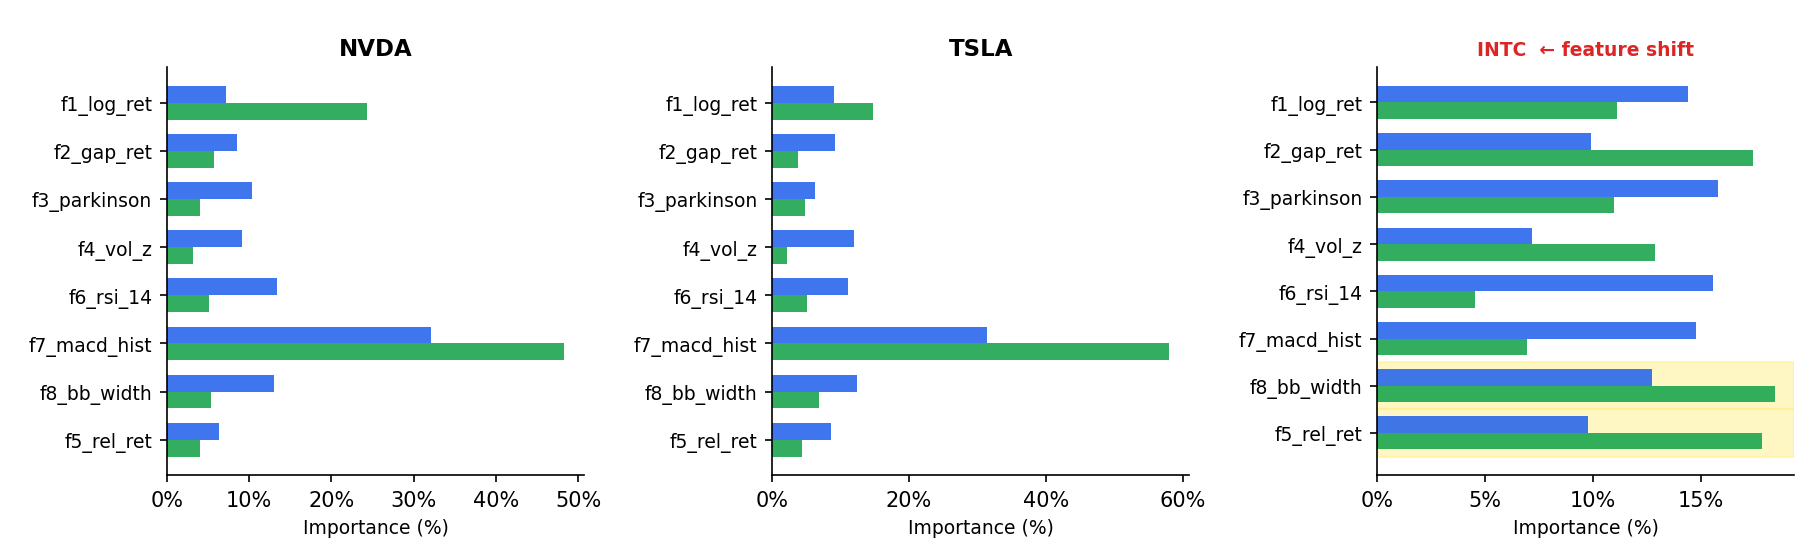
\includegraphics[width=\linewidth]{figures/ig_attribution_tickers.png}
\caption{Integrated Gradients feature attribution breakdown by ticker (NVDA, TSLA, INTC) across all analyzed events.}
\label{fig:igattribution_tickers}
\end{figure}

\begin{figure}[H]
\centering
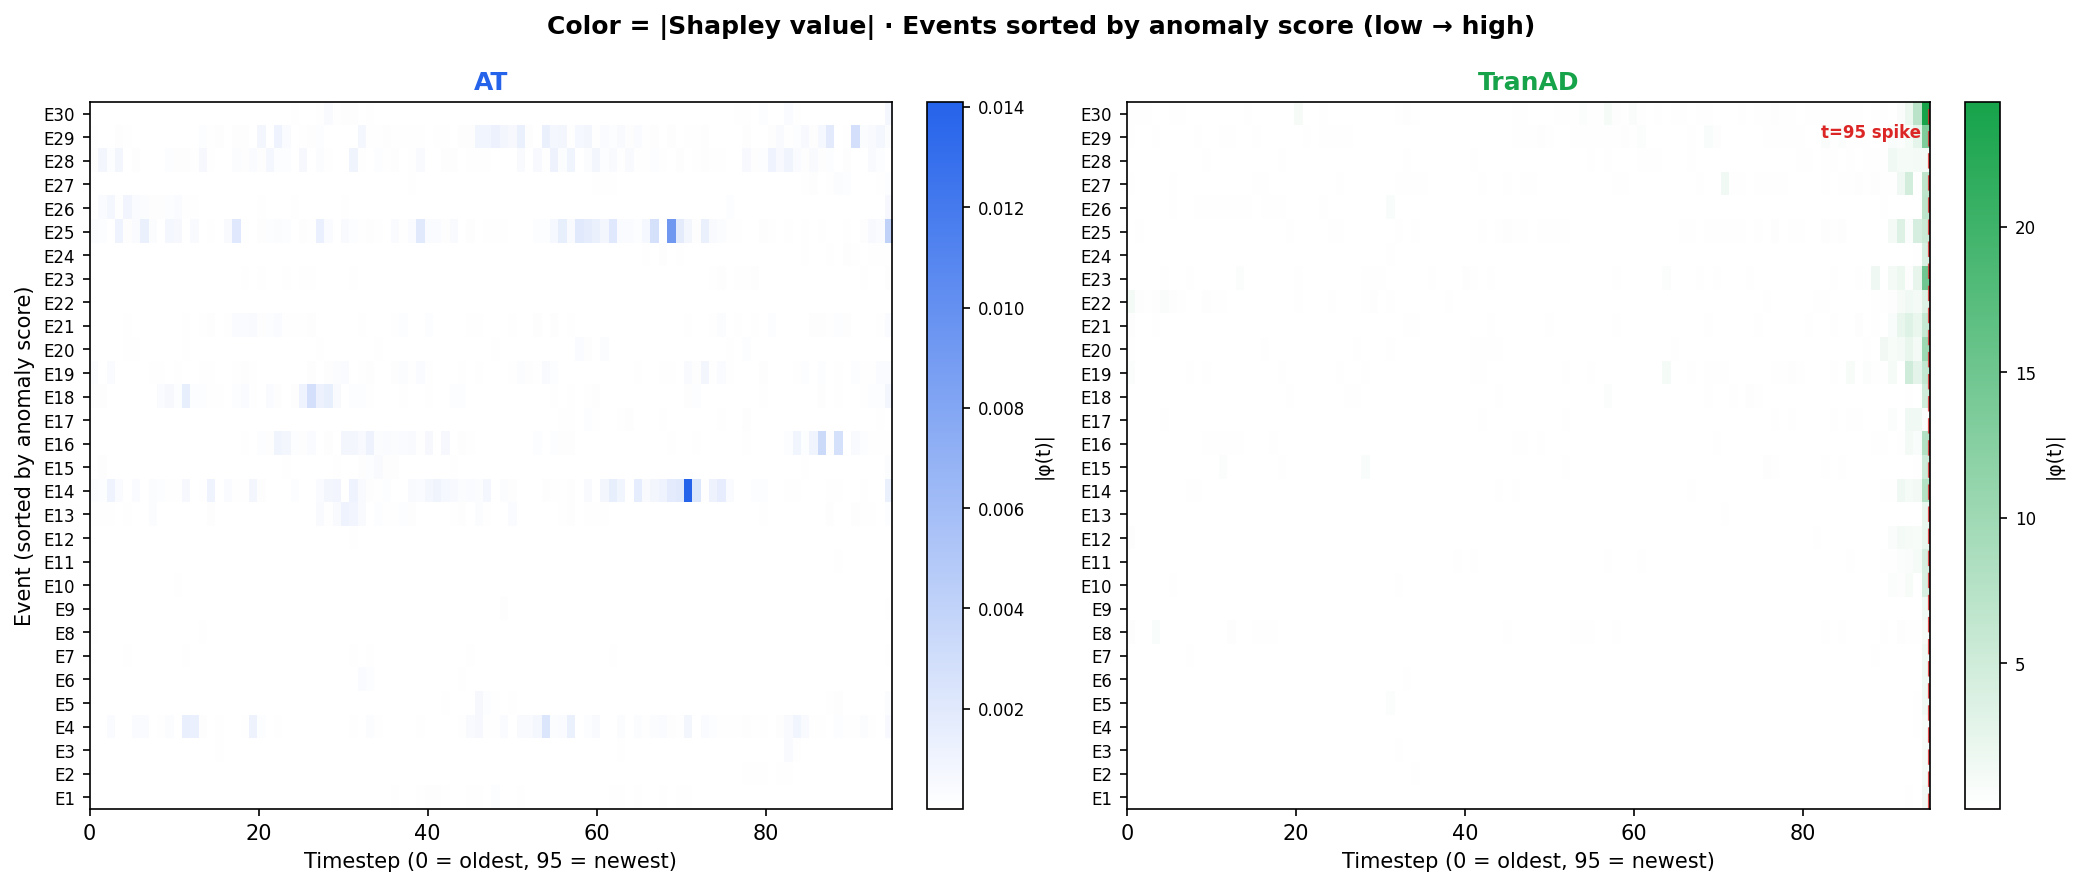
\includegraphics[width=\linewidth]{figures/timeshap_heatmap.png}
\caption{Per-event TimeSHAP temporal attribution heatmap. Color encodes $|\phi(t)|$; events are sorted by anomaly score (low $\rightarrow$ high). AT exhibits a wide dynamic range of recency concentration; TranAD shows a compressed cluster with dominant terminal-state ($t=95$) mass.}
\label{fig:timeshapheatmap}
\end{figure}

\end{document}